\begin{quote}
	\textit{``The sinister thing about a simstim construct, really, was that it carried the suggestion that any environment might be unreal, that the windows of the shopfronts she passed now with Andrea might be figments.''}
\end{quote}
\hfill \textit{Count Zero, William Gibson}
\\
\\
\\

%=========================================================================================================
%=========================================================================================================

This chapter presents the development of a preliminary PR system that combined a tablet computer, GPS, accelerometer \& magnetometer, with an OpenSim based virtual environment to allow exploration of the real world ruins of a 14th century cathedral with a virtual reconstruction of it as it stood in its prime. Cultural heritage is introduced as an ideal area for which PR systems can be applied to beneficial effect, while the accuracy of GPS tracking emerged as a constraint on this style of implementation.

%=========================================================================================================

\section{Virtual Heritage}

Alternate reality technologies have been used for over two decades~\cite{Roussou2002} to aid in the investigation, understanding \& dissemination of information pertaining to our past in the fields of archaeology \& cultural heritage. Whilst archaeology studies human activity through the recovery of remains, heritage is also concerned with intangible attributes of society; tradition, art, narratives \& other cultural evidences~\cite{Roussou2002}. \textit{Virtual heritage} is the name given to the application of advanced imaging techniques, including alternate reality techniques, to the synthesis, conservation, reproduction, representation, reprocessing \& display of this cultural evidence~\cite{roussou:photorealism}.

These techniques provide access to locations \& artefacts scattered about the world, that may reside in private collections inaccessible to scholars (much less interested amateurs) \& outwith of their original context of creation~\cite{griffin:recovering}. They allow recreations to be made of the numerous cultural heritage objects that are deteriorating or are at risk of being lost, both due to natural causes such as weather \& natural disasters but also due to acts of man such as civil war~\cite{Ikeuchi2003}.

Virtual heritage techniques offer substantial benefits to collaborative investigation of sites, where multiple users are provided the ability to collaborate via a multitude of different visualization modalities including video see-through head-tracked head mounted displays, projected table surfaces, large screen displays \& tracked hand-held displays, including the ability for experts physically located at a particular site to collaborate with those remote to it~\cite{benko:collaborative}. This combination of different techniques not only benefits experts, but has been used in the creation of contiguous platforms for building \& managing exhibitions of 3D models of artefacts accessed in museums, galleries \& via the Web~\cite{Wojciechowski2004}, focussed not only on the digitization \& subsequent interaction with such content to aid in its preservation \& protection, but also with making these resources as widely available as possible to any interested parties (scientists, archaeologists, curators, historians \& interested amateurs)~\cite{walczak:applications}.

Even traditionally two-dimensional visual resources associated with cultural heritage can be integrated into such state-of-the-art systems, visualized via immersive CAVE techniques as part of `information landscapes'~\cite{Ruffaldi2008}. Such techniques are of particular benefit to young people as cultural heritage sites often arouse little involvement in them, especially if the site's present day appearance bears few traces of its original stature \& makes it difficult to appreciate its original splendour \& importance~\cite{ardito:combining}.

%=========================================================================================================

\subsection{Alternate Reality Techniques in Virtual Heritage}

Due to the number of combinations \& diversity in approaches that have been used in the application of visualization techniques to the cultural heritage sector, attempting to comprehensively list them is impractical. Comparison via a taxonomical model that classifies approaches according to various characteristics is thus the approach adopted by Foni et al.~\cite{Foni2010} that produced the taxonomical space shown by figure \ref{taxonomy_1.png}.

\begin{figure}[h]
\centering
  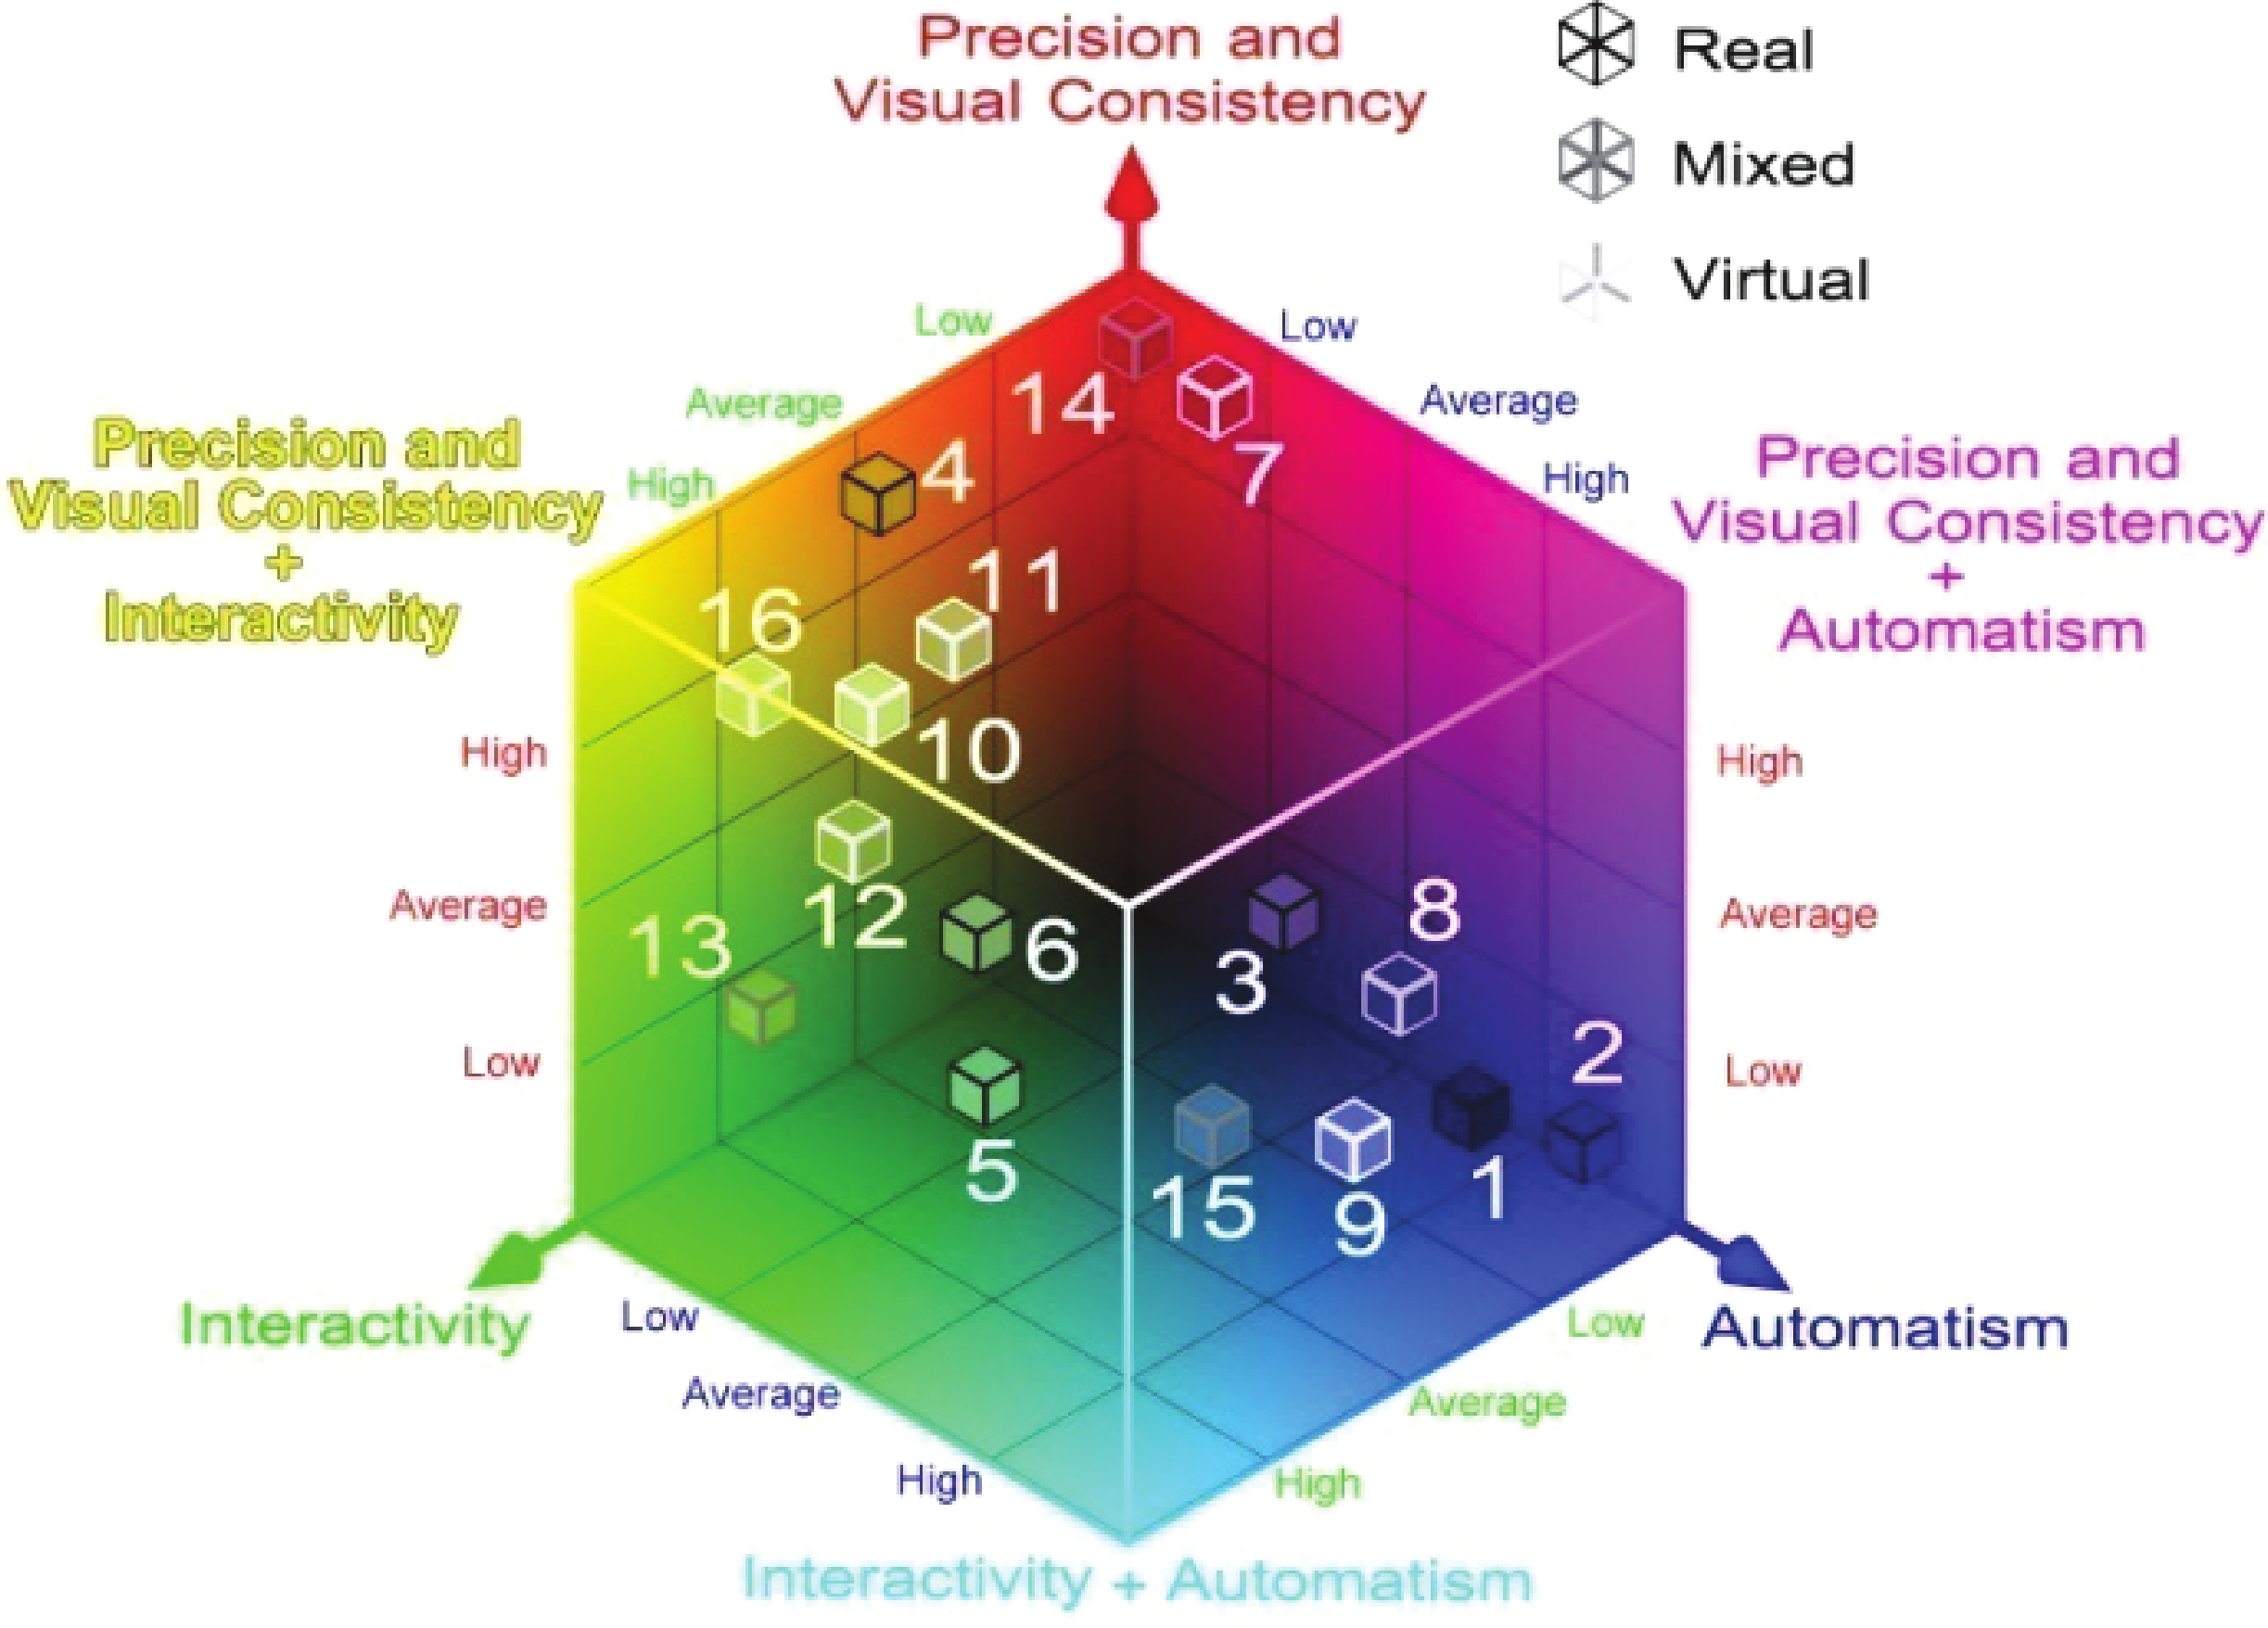
\includegraphics[width=.7\linewidth]{taxonomy_1.png}
  \caption{Taxonomical space of visualization strategies used in cultural heritage.}
  \label{taxonomy_1.png}
\end{figure}

This model classifies visualization strategies according to four continua, represented by the three physical dimensions of the 3D cube \& the degree of shading of each point within the cube. The x axis represents the level of automatism, which refers to the span of the development cycle required to produce the visualization; the y axis represents the level of precision, referring not only to the amount of geometrical detail but to all elements that can contribute to or enhance reliability; \& the z axis represents the level of interactivity, defined in this context as;

\begin{quote}
	\textit{``its capacity to contextually offer the possibility to subjectively experience an interactive behaviour in a synchronous way, thus enabling the user the opportunity to meaningfully contribute to a given experience or to affect in real time the visualized  item''}~\cite{Foni2010}.
\end{quote}

The shading of each point within the cube represents its degree of virtuality, conceptually analogous to the reality-virtuality continuum of Milgram et al. (see section \ref{milgram&kishino}) with real world/world unmodelled represented as solid black, virtual reality/world completely modelled as completely white \& positions in-between as various shades of grey. The position of 16 exemplar visualization techniques applied to cultural heritage are shown upon the cube \& explained via the table figure \ref{taxonomy_2.png}, which includes both traditional techniques \& state-of-the-art methodologies.

\begin{figure}[h]
\centering
  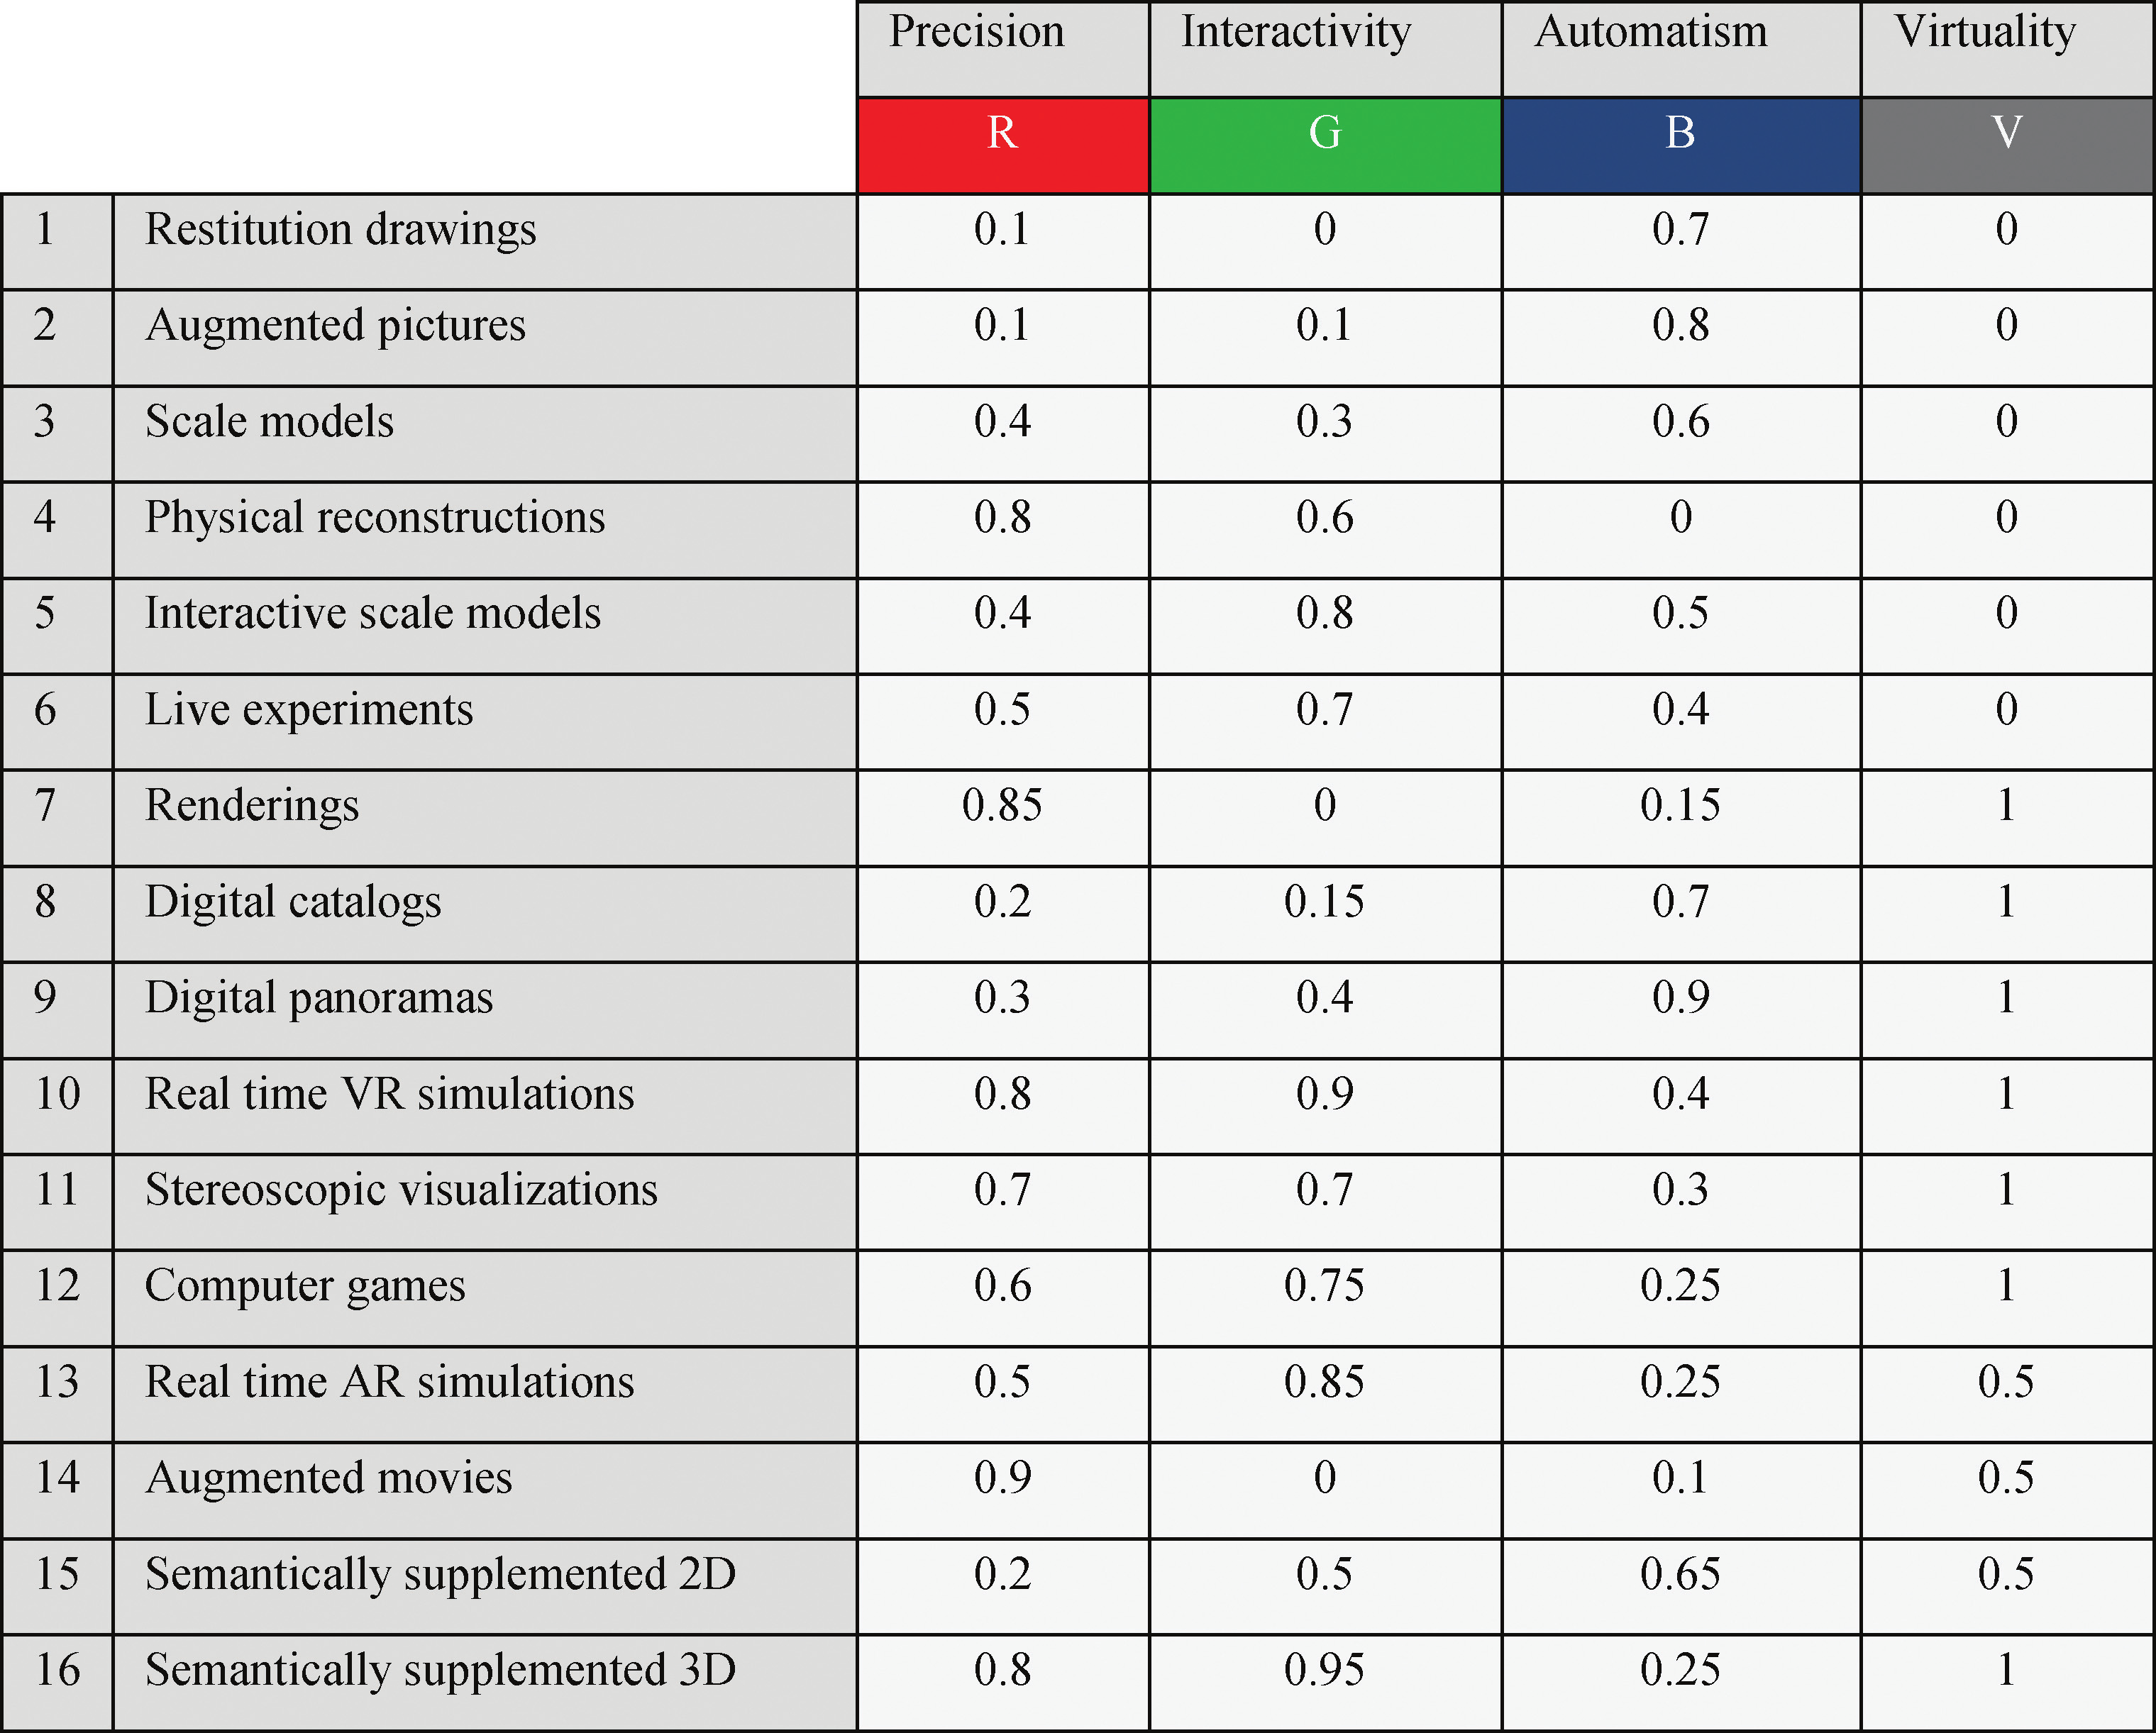
\includegraphics[width=.8\linewidth]{taxonomy_2.png}
  \caption{Coordinate sets for each approach within the taxonomical space (figure \ref{taxonomy_1.png}).}
  \label{taxonomy_2.png}
\end{figure}

%=========================================================================================================

In terms of alternate reality techniques, real time AR simulations (category 13) have been used to add artefacts, actors \& reconstructed architecture to views of present day sites that are still accessible \& may bear traces of their original status, whilst real time VR simulations (category 10) have been used to host more complete reconstructions of entire buildings \& settlements for interaction via screen, HMD \& CAVE, including where the present day site bears no evidence of its past status or is inaccessible due to latter development, change in landscape, etc..

%=========================================================================================================

The ARCHEOGUIDE project (Augmented Reality-based Cultural Heritage On-site GUIDE)~\cite{vlahakis:archeoguide} aimed to provide a `personalized electronic guide \& tour assistant' to cultural heritage site visitors. On-site help \& augmented reality reconstructions of on-site ruins were presented via a laptop, a tablet computer \& a PDA, using GPS for location tracking \& magnetometer to ascertain direction such that augmentations could be placed accordingly. The applications claimed to be supported by the platform range from archaeological research to education, multimedia publishing \& cultural tourism. The platform was prototyped at the archaeological site of Olympia, Greece.

As well as being used for walking tours, AR has been combined with the concept of telepresence to create `augmented telepresence', allowing participants to experience a `fly-through' of the ancient Nara Heijo-kyo capital of Japan, by combining aerially captured omnidirectional video augmented with related information using AR techniques~\cite{Okura2006,Okura2011}.

Augmenting views of the real world with real-time animated virtual humans has been explored by several projects, including the LIFEPLUS EU IST project, which aimed to produce `\textit{`an innovative 3D reconstruction of ancient frescos-paintings through the real-time revival of their fauna and flora, featuring groups of virtual animated characters with artificial life dramaturgical behaviors, in an immersive AR environment''}. This project pushed established augmented reality applications to the field by exploring narrative design in fictional spaces, with the aim of increasing immersion via realistic interaction, making use of captured/real-time video of a real scene~\cite{Papagiannakis2004}, presenting the visitor with \textit{``an immersive and innovative multi-sensory interactive trip to the past''}~\cite{Papagiannakis2005}. These realistic simulations of animated virtual human actors were employed in a mobile \& wearable setup, in abandonment of traditional concepts of static cultural artefacts or rigid augmentations of real world features, making use of a markerless camera tracker \& mixed reality illumination model for more consistent real-virtual \& virtual-real rendering. This platform was demonstrated in a case study on the real site of ancient Pompeii \& whilst initially targeted at the cultural heritage sector, the author(s) clarifies that as a platform it is not limited to such subjects~\cite{Papagiannakis2007}. This concept of extending rigid \& static AR with character-based event representations hopes to recreate not just discrete artefacts but the entirety of `daily life' at the scene~\cite{Papagiannakis2009}.

Although many applications of AR to cultural heritage sites are mobile in nature, using a variety of tracking techniques to localise the user \& determine their orientation, including GPS~\cite{vlahakis:archeoguide}, visual tracking of robust features of the environment~\cite{Kim2009} \& omnidirectional range sensing of a landmark database~\cite{Taketomi2011}, there are also those that present a static interface similar to coin-operated telescopes situated at popular tourist attractions~\cite{Weng2012}.

%=========================================================================================================

VR is not only useful where the real site is no longer accessible, too remote or does not bear any similarity to its original status, but also allows for more effective control over the atmospheric qualities of the environment being recreated; effects such as fog, sky, water \& particles, exploiting the latest graphical hardware by making use of shaders to deliver high quality graphics~\cite{deamicis:gamebased}. The use of a head mounted display or CAVE~\cite{cabral:x3dexperience,Christou2006} that completely blocks stimuli from the user's real world surroundings allows for this complete level of control. Unless an AR system employs various environmental monitoring techniques, the augmentations that it overlays upon the user's view of the real world will often have differing illumination than their real surroundings which has an effect upon their perceived realism~\cite{mcnamara:lightness}.

Whereas many heritage representations, architectural walkthroughs \& simulations of artefacts \& places have defined a practice where photorealism is considered an important measure of the representation's success, there is an argument that whilst such an emphasis on realism \& historical accuracy \& authenticity is important, such photorealistic methods can limit the flexibility of the reconstructions with regards to how much they can be modified \& altered to explore different reconstruction hypotheses~\cite{roussou:photorealism}. Emphasis on photorealistic graphical quality also has considerations when it comes to real time performance \& many intelligent techniques must be employed to maintain acceptable performance as complexity of reconstructions increases~\cite{willmott:largecomplex}. Particularly for dissemination to the public in museums \& visitor centres, acceptable performance is often more important than extreme historical accuracy.

%=========================================================================================================

\subsection{Virtual Heritage at the University of St Andrews}

\textbf{***Include references to Kris Getchell's thesis? Experiential learning, etc?}

The Open Virtual Worlds (OVW) research group at the School of Computer Science at the University of St Andrews has been employed in virtual heritage projects since 2007~\cite{Getchell2007}, producing a number of reconstructions of cultural heritage sites in Scotland \& further afield. These reconstructions have been produced through collaborations with academics from the university's Art History, History \& Archaeology departments, as well as with domain experts from heritage organisations including Historic Scotland \& the National Trust for Scotland. These projects range from small reconstructions of a church, to much larger reconstructions such as that of the cathedral at St Andrews which represents several years of work~\cite{Kennedy2013}. Whilst the cathedral reconstruction was completed as a research project, other reconstructions were produced specifically for use in schools in Scotland (such as Linlithgow palace, figure \ref{linlithgow_real.jpg}, \ref{linlithgow_reconstruction.png}), others for outreach purposes (Mosfell Viking farmstead, figure \ref{mosfell_outside.jpg}, \ref{mosfell_inside.jpg}) \& still others were built specifically for installation into museums (Caen Township, figure \ref{caen_township_outside.jpg}, \ref{caen_township_inside_wireframe.jpg}). Some of these reconstructions are inhabited with virtual humans that are scripted to perform certain actions specific to the role they depict at the site (figure \ref{cathedral_npc_standing.png}, \ref{cathedral_npc_talking.png}).

\TwoFig{linlithgow_real.jpg} {Linlithgow Palace today.} {linlithgow_real.jpg}
       {linlithgow_reconstruction.png} {Linlithgow Palace reconstruction.} {linlithgow_reconstruction.png}

\TwoFig{mosfell_outside.jpg} {Mosfell Viking Longhouse.} {mosfell_outside.jpg}
	   {mosfell_inside.jpg} {Longhouse interior.} {mosfell_inside.jpg}

\TwoFig{caen_township_outside.jpg} {Caen Township.} {caen_township_outside.jpg}
       {caen_township_inside_wireframe.jpg} {Caen Township wireframe detail.} {caen_township_inside_wireframe.jpg}

\TwoFig{cathedral_npc_standing.png} {Virtual humans in cathedral reconstruction.} {cathedral_npc_standing.png}
       {cathedral_npc_talking.png} {Conversing with virtual humans.} {cathedral_npc_talking.png}

These reconstructions were made using OpenSim, an open source implementation \& extension of the Second Life server which is compatible with the numerous forks of the Second Life client program. This architecture allows straightforward construction \& dissemination of the models, thanks to accessible modelling tools provided by the Second Life client itself \& the client/server model that allows the models to be accessed in various deployment scenarios including temporary deployments within controlled network \& client conditions as well as remotely via the Internet.

The reconstruction process involves the use of Geographic Information System (GIS) data from Ordnance Survey (OS) to accurately model the basic elevation of the ground. Where there is higher resolution elevation data, such as from Lidar laser surveying often employed on archaeological surveys, this is used to increase the accuracy of the resultant reconstruction. Where access to the site is possible \& depending upon development surrounding the site prior to the date being reconstructed, 360\textdegree\ panoramic photographs are captured \& then used to create a backdrop for the reconstruction, allowing identifiable aspects of the surrounding environment to improve the experience of the reconstruction. Buildings/structures are then reconstructed upon the ground layer, using numerous sources as input; satellite views, archaeological surveys, contemporary accounts, views of the site itself if relics still exist, photographic evidence, etc. Domain experts are then brought in to iteratively improve the model, commenting on aspects of the reconstruction to be altered in order to visualise a different reconstructive hypothesis.

These reconstructions have been used to host workshops at 10 schools throughout Scotland, at both primary \& secondary institutions, where all requisite computing infrastructure was taken, assembled at the school, then disassembled \& removed at the end of the day. Students are split into groups of 4-5, sharing a computer with screen, keyboard, mouse \& Xbox controller (a control modality instantly recognised by most school students). Worksheets with tasks are used to structure their interaction with the reconstructions \& guide the experiential learning experience over 20-40 minute sessions (figure \ref{linlithgow_children.jpg}). Similar workshops have also been performed in museums, using the same approach of temporary setups of computing hardware (figure \ref{musa.jpg}). In addition to traditional computer screens, larger LCD television screens \& still larger projection screens, Oculus Rift VR headsets have been used with this same content~\ref{rift_exhibition.jpg}.

In addition to these temporary workshops, the reconstructions have also been used in permanently installed exhibits in museums \& visitor centres, including the Virtual Time Travel Project (VTTP), which combines multi-head projection with Natural User Interaction (NUI) via Microsoft Kinect, which has been installed at the Timespan Museum \& Arts Centre in Helmsdale, allowing visitors to explore the reconstruction of the Caen Township by using simple gestures, instead of relying upon a keyboard, game controller or other traditional interface (figure \ref{VTTP_projection.png}).

\TwoFig{linlithgow_children.jpg} {School students learning via a reconstruction.} {linlithgow_children.jpg}
       {VTTP_projection.png} {VTTP installation at Timespan.} {VTTP_projection.png}

\TwoFig{rift_exhibition.jpg} {OVW via Oculus Rift.} {rift_exhibition.jpg}
       {musa.jpg} {Museum workshop.} {musa.jpg}

%=========================================================================================================

\section{Parallel Reality in Virtual Heritage}
Applications of alternate reality techniques within virtual heritage have thus far broadly fallen into the categories of AR, experienced at the site, or VR, experienced away from the site (in terms of space, time, or both). The dissemination of the OVW group's content has been no exception to this observation, falling into categories 10-12 of figure \ref{taxonomy_2.png}, with complete virtual environments that are experienced with both spatial \& temporal separation from the real site that they represent.

Applying the concept of parallel reality to virtual heritage represents an opportunity to explore an exciting new modality of interaction that combines the complete virtual environments of categories 10-12 with the real time juxtaposition between real \& virtual environments of AR systems from category 13. In terms of the four categories of the taxonomic space, such a PR system would combine the high precision \& interactivity of a VR system (category 10) with two values of viruality, as the user is provided the ability to observe either the complete virtual environment (virtuality = 1) or the unmodified real environment (virtuality = 0). The automatism of such a system would occupy a position between that of VR \& AR; whilst the system will require a more involved development cycle than a purely VR one, the slackened requirements on registrational accuracy of a PR system compared to an AR system promise higher automatism than a purely AR system.

%=========================================================================================================

\section{The Virtual Time Window}
The Virtual Time Window (VTW) is an application of parallel reality to virtual heritage, leveraging the OVW group's existing OpenSim virtual reconstructions of cultural heritage sites in a handheld package that allows tandem exploration of both the real cultural heritage sites \& their spatially equivalent virtual reconstructions.

VTW manifests as a tablet computer which is capable of tracking its position via GPS, its compass heading via magnetometer (`electronic compass') \& its pitch via accelerometer. Existing AR projects have proven through application the suitability of smartphones \& tablets for mobile, position \& orientation aware applications that present virtual content within a cultural heritage context. These devices are also entering ubiquity today \& thus present a platform that can be quickly assimilated by most users. The tablet runs a modified version of the Second Life client in order to access, via wifi, a virtual reconstruction of a cultural heritage site hosted by an OpenSim server. The Second Life client is controlled entirely by the tablet's position \& orientation - the user does not manually control any aspect. The modality of interaction offered is similar to that of using a smartphone to take a photograph, but whereas the screen of the smartphone shows the real environment as it is, the screen of the VTW tablet shows the environment as it was in the past - a window to the past, or \textit{Virtual Time Window}. The user is free to explore the real cultural heritage site, observing it in its current state, whilst at any moment `looking through' VTW to see what a particular vantage looked like in the past. See figure \ref{vtw_high_level.png} for a representation of the components of the platform at the conceptual level.

\begin{figure}[h]
\centering
  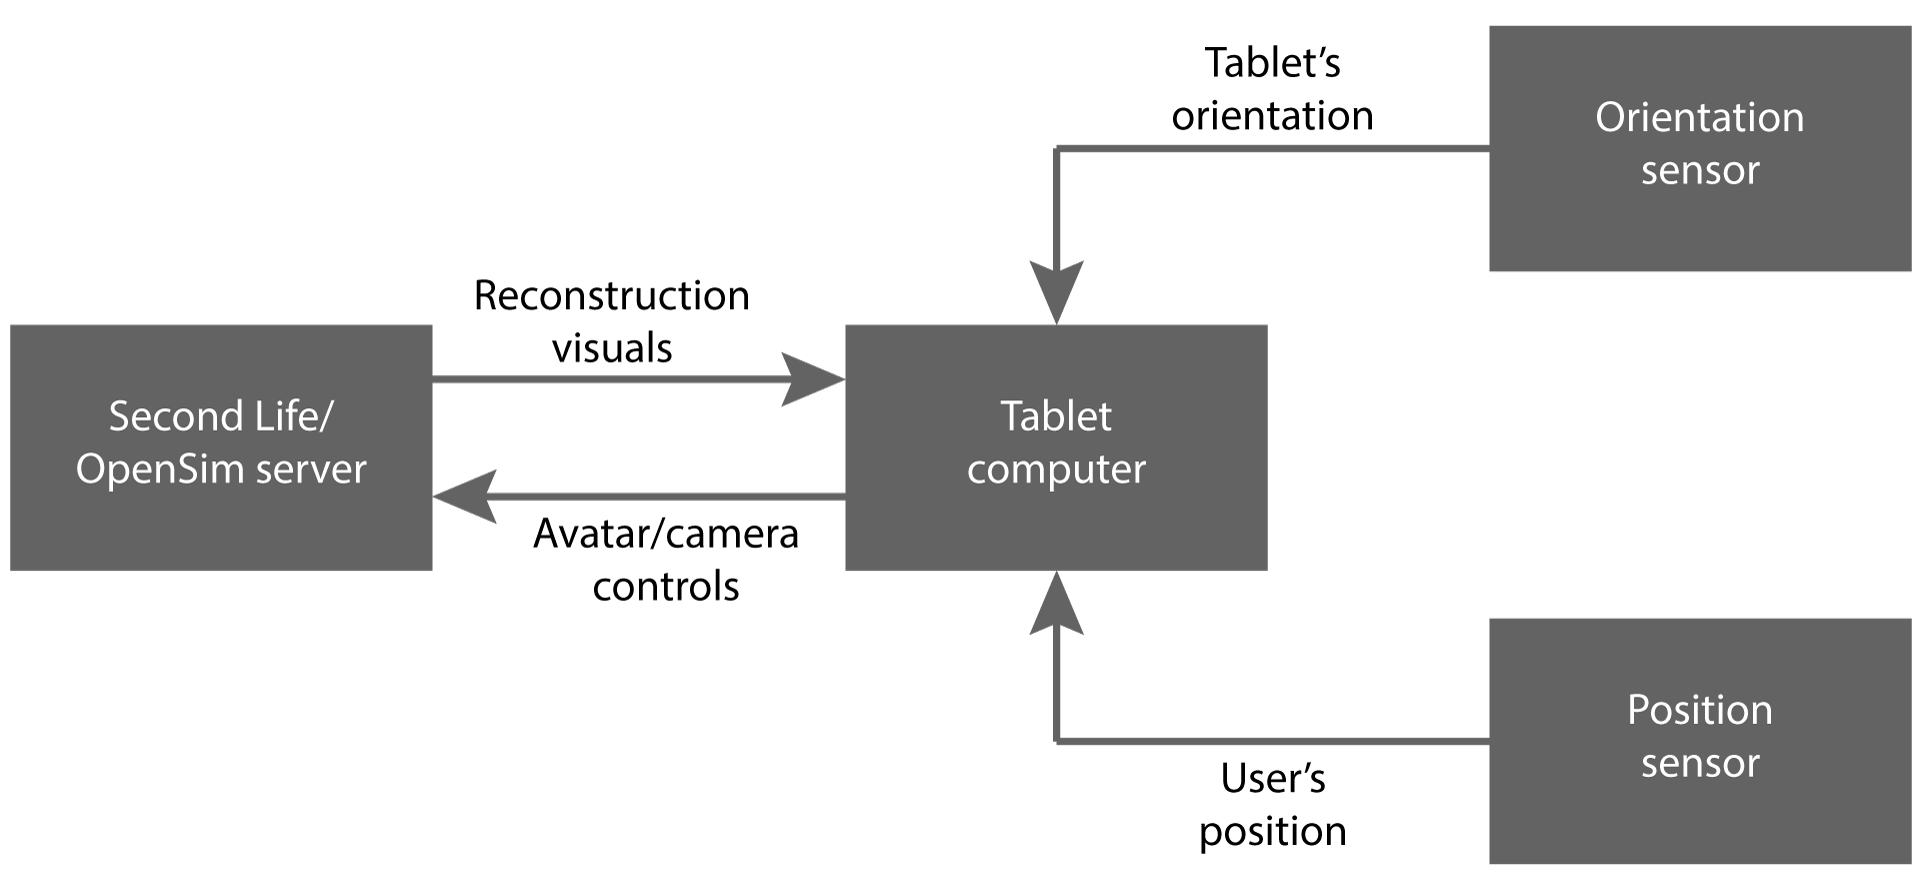
\includegraphics[width=.7\linewidth]{vtw_high_level.png}
  \caption{High level architecture of VTW.}
  \label{vtw_high_level.png}
\end{figure}

In terms of the combined Milgram/Waterworth model, the displacement along the locus axis when the user switches their attention between their real environment \& the virtual environment upon the tablet will displace less toward the VR extremum than shown in figure \ref{focus-locus-sensus-with-virtuality-continuum-with-transition} which represents transitions between real \& virtual environments when using a HMD that effectively blocks all stimuli from the real world when observing the virtual. When considering the environmental provision, VTW features two complete environments, one real \& the other virtual. From the perspective of transitioning between receiving stimuli from each environment, there is an obvious difference between VTW's tablet based approach compared to a HMD approach, as the latter effectively forces all percepts to emanate from one environment whilst the former allows percepts emanating from both environments to be perceived simultaneously.

Whilst this will intuitively make transitions easier to perform \& create less risk of a jarring Gestalt switch, it will also intuitively limit the intensity of the sense of presence attainable in the virtual environment as the sense of `looking in to' the virtual environment will always leave the user readily aware of the real environment surrounding them. Whilst VTW is a PR system, one might liken the experience of interacting with it to be similar to that of an AR system.

%Map showing spatial separation of Madras \& cathedral?

%How with VTW we have a small `window' into the virtual, which is then surrounded by the real. So unlike Mirrorshades which is about distributing attention by time (one environment, then the other), VTW is about distributing attention by gaze/place (different parts of a single view/combined environment).

%=========================================================================================================

\subsection{Second Life \& Mobility}

\label{SecondLifeMobility}

\newcommand{\LumiyaFootnote}{\footnote{\url{https://play.google.com/store/apps/details?id=com.lumiyaviewer.lumiya&hl=en_GB}}}

\newcommand{\WindpadFootnote}{\footnote{\url{http://www.msi.com/product/windpad/WindPad-110W.html}}}

%=====================

At the time of the VTW project (Summer 2012) the only fully-featured Second Life clients available were for x86 platforms. Whilst the Android client Lumiya\LumiyaFootnote{} was available, it was in its earliest stages \& very limited in its features \& usability. This limited the choice of tablet to those few x86 models that had reached market, with the MSI WindPad 110W\WindpadFootnote{} presenting the most promising solution: a 10'' tablet sporting an AMD Brazos Z01 APU (combining a dual-core x86 CPU with a Radeon HD6250 GPU).

The Second Life client, intended for use on a desktop or laptop computer, provides provision for controlling the avatar's position \& the camera orientation by keyboard, mouse \& joystick. For the purposes of VTW, this position \& orientation control must be tied to the physical position \& orientation of the tablet itself. To this end, it is necessary to make use of various sensors connected to the tablet (either internally, or externally) \& to interface these with the Second Life client in such a way that it can make use of their collected data to appropriately control the avatar's position \& camera orientation.

%\cite{willmott:largecomplex} occlusion culling etc., missing in Second Life/OpenSim

%Talk about history of Second Life/OpenSim in academia/research, including original cross reality research.

%The 3D virtual environment component of the Pangolin system was implemented using the Second Life/OpenSimulator (SL/OpenSim) platform, which provides a 3D social-oriented multi-user non-competitive virtual environment which focuses on the community, creation and commerce~\cite{Sevan2008} aspects of many users interacting within a shared space through the abstraction of avatars, rather than the competitive natures of games and the solitary environments commonly afforded by simulation and visualization platforms.

%The distributed client/server model of SL/OpenSim, wherein 3D content is stored on a grid of servers operated by a multitude of organizations and distributed to and navigated between by dispersed clients on demand when they enter a particular region rather than being pre-distributed as is the norm for games, simulations and visualizations, is analogous to the manner in which 2D social Web content is served from Web servers to client browsers and apps.

%This style of content delivery is necessary when considering the dynamic and ephemeral nature of consumer-generated media which constitutes the majority of the current 2D social Web and will make up the majority of expanding 3D social Web content.

%=========================================================================================================

\section{Orientation Control}

\label{OrientationControl}

\newcommand{\ArduinoFootnote}{\footnote{\url{http://www.arduino.cc/}}}

\newcommand{\MMAfootnote}{\footnote{\url{http://cache.freescale.com/files/sensors/doc/data_sheet/MMA8452Q.pdf}}}

\newcommand{\ADXLfootnote}{\footnote{\url{http://www.analog.com/static/imported-files/data_sheets/ADXL335.pdf}}}

\newcommand{\HMCfootnote}{\footnote{\url{http://www51.honeywell.com/aero/common/documents/myaerospacecatalog-documents/Defense_Brochures-documents/HMC5883L_3-Axis_Digital_Compass_IC.pdf}}}

\newcommand{\HMCtwoFootnote}{\footnote{\url{http://www51.honeywell.com/aero/common/documents/myaerospacecatalog-documents/Missiles-Munitions/HMC6343.pdf}}}

\newcommand{\HMCvccFootnote}{\footnote{The HMC6343 requires 2.7 to 3.6V input on VCC/VDD, this table showing connection to 5V assumes a HMC6343 breakout with appropriate step down.}}

\newcommand{\itwocFootnote}{\footnote{The HMC6343's I2C lines must be pulled up to 3.3V, this table shows connection to an Arduino Uno R3's I2C lines which are pulled up to 5V assuming a HMC6343 breakout with appropriate level shifters.}}

%http://www.nxp.com/documents/user_manual/UM10204.pdf

%=====================

In order to control Second Life's camera in the fashion required of VTW, sensor data are required for the orientation in which the user is holding the tablet. Specifically, the tablet's yaw \& pitch are needed; roll is less important as it is conceived that the user will generally hold the tablet roughly level with the horizon when looking `through' it.

VTW considers yaw in terms of magnetic compass bearing, as this provides a value that can be used to directly control the yaw of the virtual camera while the virtual reconstruction within OpenSim is correctly oriented to OpenSim's own compass. Magnetic compass bearings are sensed electronically via a 3-axis microelectromechanical (MEMS) magnetometer, which measures the strength of magnetic field being experienced along each of its 3 axes. By comparing the values of each axis to the known direction of the field lines of Earth's magnetic field, a compass bearing relative to the magnetometer's orientation can be calculated. Pitch is sensed using a 3-axis MEMS accelerometer, which measures force of acceleration along each of its 3 axes. In the case of static or slow moving applications, this acceleration is predominantly that caused by the Earth's gravitational pull \& by comparing the values of each axis the direction of this acceleration (down toward the centre of the Earth) can be determined in relation to the orientation of the accelerometer itself \& thus the accelerometer's own orientation can be deduced.

Due to the fact that the WindPad tablet does not feature a built-in magnetometer \& its built-in accelerometer is little more than a rudimentary tilt sensor for differentiating between discrete cases of landscape and portrait orientation for screen rotation, it was necessary to interface external magnetometer \& accelerometer sensors. The popular Arduino\ArduinoFootnote{} microcontroller platform was used for prototyping with several different sensor packages, including the MMA8452\MMAfootnote{}, the ADXL335\ADXLfootnote{} \& the HMC5883L\HMCfootnote{}. The package adopted for use with VTW from this prototyping stage was the HMC6343\HMCtwoFootnote{}, which combines a 3-axis MEMS magnetometer \& 3-axis MEMs accelerometer into a single package sporting an I2C interface, along with algorithms to internally apply the accelerometer's readings to `tilt compensate' the magnetometer's readings. Figure \ref{arduino_wiring_hmc.png} provides a wiring diagram for connectivity of a HMC6343 to an Arduino Uno R3, with the pinout values provided by figure \ref{HMC6343wiringtable} \& Figure \ref{arduino_joystick_for_second_life_1.jpg} shows an assembled unit.

\begin{figure}[h]
\centering
  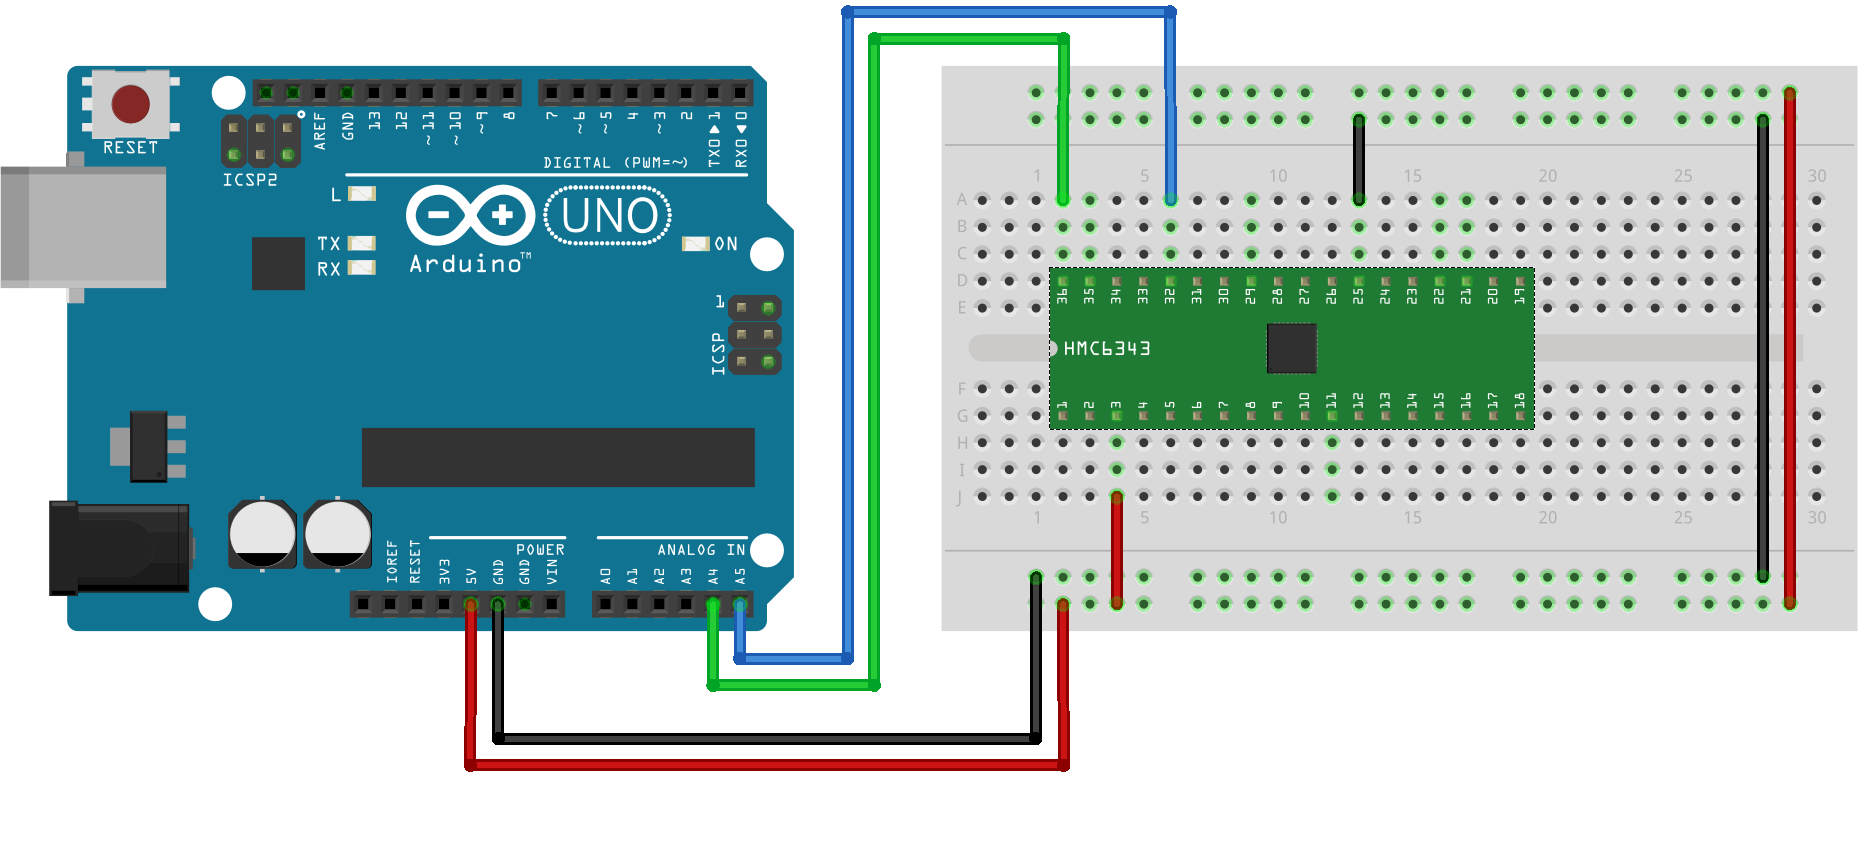
\includegraphics[width=\linewidth]{arduino_wiring_hmc.png}
  \caption{Example wiring for Arduino with HMC6343 for joystick operation.}
  \label{arduino_wiring_hmc.png}
\end{figure}

%=====================

\begin{figure}[h]
\begin{center}
\begin{minipage}{.7\linewidth}
\begin{center}
%\begin{tabularx}{250pt}{|>{\centering\arraybackslash}X|>{\centering\arraybackslash}X|}
\begin{tabular}{| c | c |}
\hline	
\textbf{HMC6343 pin} & \textbf{Arduino Uno R3 pin} \\
\hline
VCC & 5V\HMCvccFootnote{} \\
\hline
GND & GND \\
\hline
SDA & A4\itwocFootnote{} \\
\hline
SCL & A5 \\
\hline
\end{tabular}
\end{center}
\end{minipage}
\end{center}
\caption{Pin designation for figure \ref{arduino_wiring_hmc.png}.}
\label{HMC6343wiringtable}
\end{figure}

%=====================

\begin{figure}[h]
\centering
  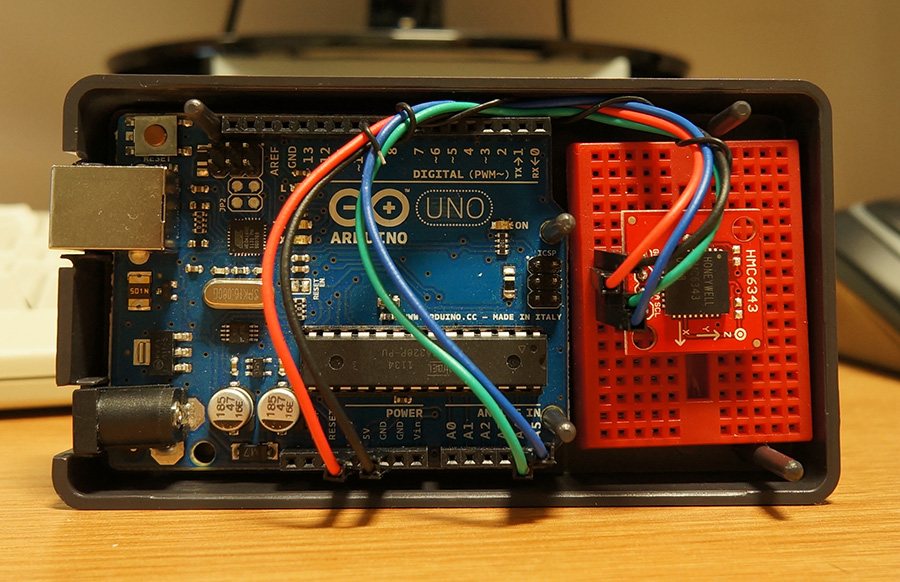
\includegraphics[width=.6\linewidth]{arduino_joystick_for_second_life_1.jpg}
  \caption{Assembled Arduino Uno R3 + HMC6343.}
  \label{arduino_joystick_for_second_life_1.jpg}
\end{figure}

A magnetometer used alone is only capable of providing a meaningful compass bearing when held level. In the case of applications where a compass bearing is required of a device that is not maintained level, such as in the case of VTW, the non-level orientation of the device must be taken into account to offset the readings of the magnetometer \& provide a correct compass bearing. The HMC6343's combination of magnetometer, accelerometer \& algorithms provides a single package that internally performs this process, using the readings from its accelerometer to compensate the readings from its magnetometer \& provide a meaningful compass bearing in non-level orientations.

Further requirements for obtaining accurate compass bearings from a MEMS magnetometer are to account for distortions to the magnetic field it senses \& to compensate the bearings it reports for the amount of magnetic declination for the location \& date wherein it is being used. Various materials that influence magnetic fields or produce their own magnetic field will distort the Earth's magnetic field \& thus impact the readings that a MEMS magnetometer collects. In the case of VTW, the sources of primary consideration are the electronics of the Arduino, tablet \& associated wiring. Due to the nature of these sources \& the fact that they are permanently situated \& attached to the same frame of reference as the magnetometer, moving as it moves, the distortions can be mitigated using a hard iron offset approach. Magnetic declination refers to the difference between `magnetic north' \& geographic `true north'. This value varies depending upon world location \& changes over time, so must be updated when the magnetometer is deployed to a different location or used at a subsequent date.

%***Reference for hard iron offset - here or later where we talk about the hex?

%=========================================================================================================

\subsection{Exploiting Second Life's Joystick Support}

\label{exploitJoystick}

\newcommand{\ArduinoJoystickVideoFootnote}{\footnote{\url{https://www.youtube.com/watch?v=-ddtmqoGNmg}}}

\newcommand{\atmegaFootnote}{\footnote{\url{http://www.atmel.com/devices/ATMEGA16U2.aspx}}}

\newcommand{\atmegaTFootnote}{\footnote{\url{http://www.atmel.com/devices/atmega328.aspx}}}

\newcommand{\arduinousbhidFootnote}{\footnote{\url{http://hunt.net.nz/users/darran/weblog/a3599/}}}

\newcommand{\lufaFootnote}{\footnote{\url{http://www.fourwalledcubicle.com/LUFA.php}}}

%=====================

As highlighted in section \ref{SecondLifeMobility} the Second Life client can be controlled only via mouse, keyboard \& joystick. Using the HMC6343's compass bearing \& yaw values therefore requires one of two approaches;

\begin{enumerate}
	\item Encapsulating the compass bearing \& yaw values into mouse, keyboard \&/or joystick commands;
	\item Modification to the Second Life client to allow the compass bearing \& yaw values to be used directly at a lower level of abstraction.
\end{enumerate}

Method 1 has the advantage of having no reliance upon any particular Second Life client, as all available clients are forks of the official client from Linden Lab \& maintain the same keyboard, mouse \& joystick interfaces. However if the level of control attainable by re-purposing these interfaces for control from magnetometer \& accelerometer data is not enough, method 2 will be the only option.

Conceptually, all Arduino boards are programmed over an RS-232 serial connection. When the platform was first launched, the Arduino boards themselves had a physical DE-9 serial connector with which to connect to a host computer's serial connector. But as serial connectors all but disappeared from modern computers, the Arduino's serial connector was replaced in later revisions with a USB connector, as USB is now all but ubiquitous on today's computers. The move from a physical RS-232 connector to a USB connector requires additional hardware upon the Arduino board to convert between RS-232 \& USB, as the ATMega328\atmegaTFootnote{} microcontroller at the heart of the Arduino Uno R3 does not have a USB interface itself. For this reason the current revision, the Arduino Uno R3, sports an ATMega16U2\atmegaFootnote{} microcontroller that serves to convert communications between the two standards, RS-232 \& USB.

With its stock firmware, the Arduino's ATMega16U2 presents itself to the host computer as a USB-to-serial bridge. However the ATMega16U2 can have this stock firmware replaced in order to change its behaviour. One of these new behaviours is to act as a USB Human Interface Device (HID) class controller, identifying itself to the host computer as one of a myriad input devices - including joysticks. Using a USB HID class joystick firmware for the ATMega16U2\arduinousbhidFootnote{}, based upon the Lightweight USB Framework for AVRs (LUFA)\lufaFootnote{}, the Arduino can imitate a standard USB joystick, sending joystick commands to the host computer using the protocol in the USB specification.

%***How to flash the firmware

In this manner, the Arduino can marshal the values obtained from the HMC6343 into standard USB HID joystick commands, allowing the Second Life client's stock joystick interface (see figure \ref{arduino_joystick_for_second_life_3.jpg}) to be used to control the camera orientation (\& avatar movement) according to the physical orientation of the HMC6343, as can be seen in\ArduinoJoystickVideoFootnote{}.

\begin{figure}[h]
\centering
  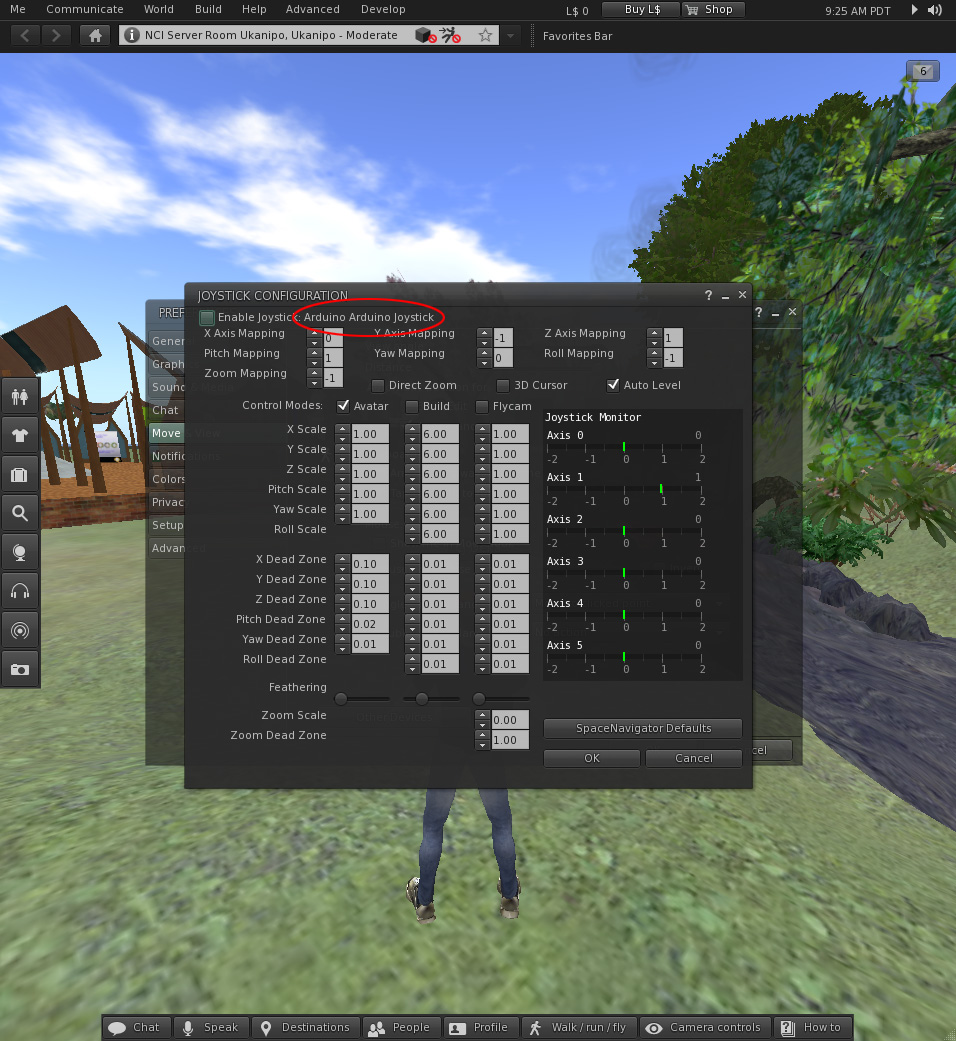
\includegraphics[width=.7\linewidth]{arduino_joystick_for_second_life_3.jpg}
  \caption{Configuration in Second Life client for Arduino + HMC6343 `joystick'.}
  \label{arduino_joystick_for_second_life_3.jpg}
\end{figure}

Unfortunately, the precision attainable through this approach is not sufficient for the style of control \& interaction required for VTW. Specifically, the Second Life client's joystick interface applies smoothing/damping to the joystick inputs, preventing reliable rotations or movements of specific values - sending a joystick command to rotate the camera by $x$\textdegree\ followed by a second command to rotate the camera by $-x$\textdegree\ does not reliably return the camera to its original orientation before the application of the first rotation. As the interaction required is to map the \textit{absolute} orientation of the tablet to the Second Life camera, this discrepancy (which cannot be disabled from the Second Life client's joystick configuration) renders the approach unworkable.

%=========================================================================================================

\section{Position Control}
In order to control the position of the Second Life avatar, sensor data are required for the position of the user in the real world. As the cultural heritage sites that VTW was intended for use upon are outdoor sites, namely those where there are traces of ruins \& clear views of the sky, GPS is the logical choice for tracking user position. GPS has been widely used as a localization technique within virtual heritage, particularly for AR applications.

%***diagram showing this

In order for readings from a GPS receiver to be used to control the position of the Second Life avatar within a reconstruction, a translation must be performed between the coordinate system of GPS (latitude \& longitude) \& the coordinate system of Second Life (simple X,Y coordinates within 256 metre square `regions'). This is achieved by use of a single `anchor point', for which both the real world latitude \& longitude \& the corresponding virtual world X,Y coordinates are known. Calculating Second Life displacement from these X,Y coordinates is achieved by applying the scale of the reconstruction to the displacement between the anchor point's latitude \& longitude \& the user's current position reported as latitude \& longitude by a GPS receiver. This real world displacement is calculated using the haversine formula~\cite{VanBrummelen2012}, which is used to calculate the `great circle' (orthodromic) distance between two points on the surface of a sphere (such as the Earth, when simplified from its oblate spheroid shape). The central angle \text{$\left(\frac{d}{r}\right)$} between the two points is given by;

\begin{equation}
\label{haversine1}
\text{haversin}\left(\frac{d}{r}\right) = \text{haversin}(\phi_{2}-\phi_{1})+\cos(\phi_{1})\cos(\phi_{2})\text{haversin}(\lambda_{2}-\lambda_{1})
\end{equation}

where;

\begin{itemize}
	\item \text{haversin} is the haversine function
		\begin{equation}
		\label{harsine2}
			\text{haversin}(\theta) = \sin^{2}\left( \frac{\theta}{2}\right) = \frac{1-\cos(\theta)}{2}
		\end{equation}
	\item $d$ is the distance between the two points along a great circle of the sphere,
	\item $r$ is the radius of the sphere,
	\item \text{$\phi_{1},\phi_{2}$} are the latitudes of point 1 \& point 2,
	\item \text{$\lambda_{1},\lambda_{2}$} are the longitudes of point 1 \& point 2.
\end{itemize}

The equation can be solved for the distance $d$ by applying the inverse haversine function or through application of arcsine;

\begin{equation}
	\label{haversine3}
	d = r\;\text{haversin}^{-1}\left( h \right) = 2r \arcsin \left( \sqrt{h} \right)
\end{equation}

where $h$ is $\text{haversin}\left( \frac{d}{r} \right)$;

\begin{align}
d & = 2r \arcsin\left( \sqrt{\text{haversin} \left( \phi_{2} - \phi_{1} \right) + \cos \left( \phi_{1} \right) \cos  \left( \phi_{2} \right) \text{haversin} \left( \lambda_{2} - \lambda_{1} \right) } \right) \nonumber \\ 
& = 2r \arcsin\left( \sqrt{\sin^{2} \left( \frac{\phi_{2} - \phi_{1}}{2}\right) + \cos\left( \phi_{1} \right) \cos\left( \phi_{2} \right) \sin^{2} \left( \frac{\lambda_{2} - \lambda_{1}}{2} \right) } \right)
\end{align}

The prerequisites for this approach are that the Second Life model is aligned correctly to the Second Life compass as the real location is aligned to real bearings (also required for orientation control from the previous section), a single anchor point for which both the real world latitude \& longitude \& the corresponding virtual world X \& Y coordinates are known \& that the reconstruction adheres to a known, consistent scale.

Figure \ref{haversine_example.png} illustrates this arrangement. In the real world, on the left, we know the latitude \& longitude of the anchor point, as well as the latitude \& longitude of the user's current position as reported by the GPS receiver. In the virtual world, on the right, we know the X,Y coordinates that are equivalent to the latitude \& longitude of the anchor point \& we must calculate the X,Y coordinates that are equivalent to the user's current position as reported by the GPS receiver.

\begin{figure}[h]
\centering
  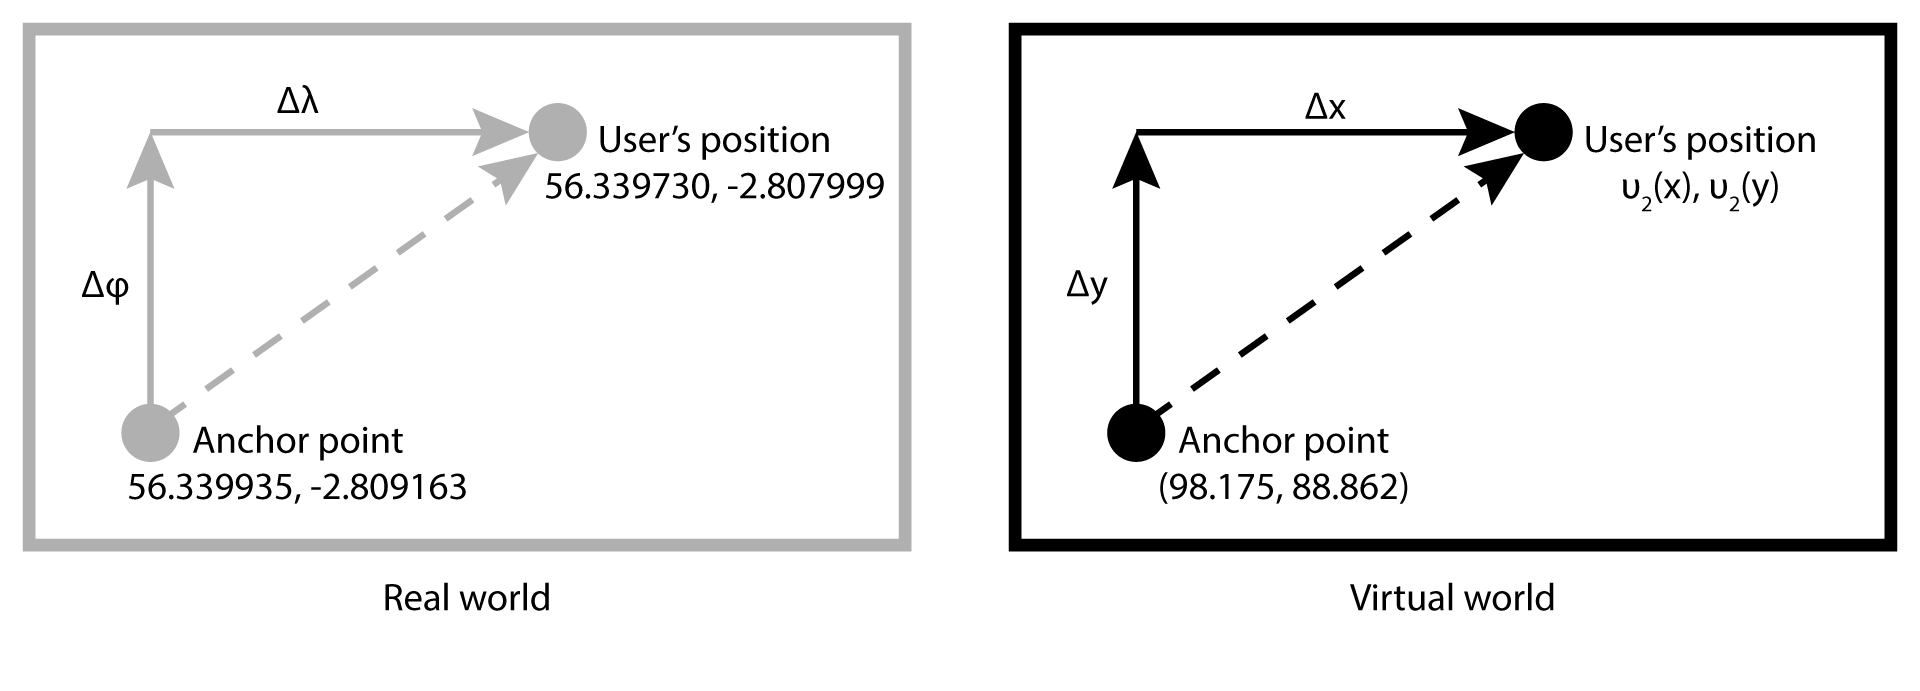
\includegraphics[width=\linewidth]{haversine_example.png}
  \caption{Using haversine to mimic real world movement in a virtual world.}
  \label{haversine_example.png}
\end{figure}

The difference in longitude between the anchor point \& the user's position, $\Delta\lambda$, is given by;

\begin{equation}
2r \arcsin\left( \sqrt{\sin^{2} \left( \frac{\lambda_{2} - \lambda_{1}}{2} \right) } \right)
\end{equation}

While the difference in latitude between the anchor point \& the user's position, $\Delta\phi$, is given by;

\begin{equation}
2r \arcsin\left( \sqrt{\sin^{2} \left( \frac{\phi_{2} - \phi_{1}}{2}\right)} \right)
\end{equation}

Applying the scale of the reconstruction to these values gives $\Delta$x \& $\Delta$y, which can then be added or subtracted from the X,Y coordinates of the anchor point to give the coordinates of the user's position, $\upsilon_{2}(x),\upsilon_{2}(y)$.

%Using the haversine formula the great-circle (or orthodromic) distance between the latitude of the anchor point and the latitude of the new GPS reading is calculated, then applying the scale of the model results in the equivalent distance in OpenSim metrics between the Y coordinate of the anchor point and the Y coordinate of the position corresponding to the new GPS reading. Repeating the same calculations with the longitude of the new GPS reading provides the distance between the X coordinate of the anchor point and the X coordinate of the position corresponding to the new GPS reading. Adding or subtracting these distances as appropriate to the OpenSim coordinates of the anchor point provides the OpenSim coordinates that correspond to the new GPS reading, to which the avatar is then instructed to move.

%The anchor point is specified using global coordinates, not local coordinates. This allows navigation to operate across region boundaries and within mega regions (it is not limited to a single 256x256 meter OpenSim region) and there are no restrictions for the placement of the OpenSim component of the anchor point (it can be anywhere in any region, movement of the avatar can be in any direction from it (positive and negative), it does not have to be at the center of the model or even in a region that the model occupies).

%Calculating a global coordinate is simply a case of multiplying the position of the region by 256 and then adding the local coordinate. For example, for an anchor at local coordinate $(127,203,23)$ within a region that is at $(1020,1042)$ the global X coordinate is calculated as $(1020 * 256) + 127 = 261247$ and the global Y coordinate as $(1043 * 256) + 203 = 267211$. Elevation (Z) is ignored due to a combination of the relatively low accuracy of these data attainable via GPS (when compared to the longitudinal/latitudinal accuracy) and as the case study explored involved users navigating outdoor ruins remaining at ground level.

%=========================================================================================================

\subsection{GPS Receivers}

\newcommand{\azurewaveFootnote}{\footnote{\url{http://www.azurewave.com/product_GPS-M19_1.asp}}}

\newcommand{\habFootnote}{\footnote{\url{http://ukhas.org.uk/}}}

\newcommand{\ubloxFootnote}{\footnote{\url{https://u-blox.com/en/gps-modules/pvt-modules/previous-generations/max-6.html}}}

\newcommand{\sarantelFootnote}{\footnote{\url{http://www.sarantel.com/sl1200_(33).html}}}

\newcommand{\MAXvccFootnote}{\footnote{The MAX-6 requires 2.5 to 3.6V input on VCC, this table showing connection to 5V assumes a MAX-6 breakout with appropriate step down.}}

\newcommand{\MAXserialFootnote}{\footnote{The data pins of the MAX-6 need to be pulled up to between 0.7 to 1.0 of the supply to VCC, so a breakout with appropriate level shifters is required for connection directly to an Ardunio Uno R3's 5V digital pins.}}

\newcommand{\softwareserialFootnote}{\footnote{\url{http://arduino.cc/en/Reference/SoftwareSerial}}}

\newcommand{\maxProtocolFootnote}{\footnote{\url{https://u-blox.com/images/downloads/Product_Docs/u-blox6_ReceiverDescriptionProtocolSpec_(GPS.G6-SW-10018).pdf}}}

\newcommand{\tinygpsFootnote}{\footnote{\url{http://arduiniana.org/libraries/tinygps/}}}

%=====================

The WindPad features an internal AzureWave GPS-M16 GPS receiver\azurewaveFootnote{}, however poor API provision and meagre documentation required the adoption of an alternative receiver. As an Arduino was already being used to provide orientation data from accelerometer \& magnetometer, integrating the GPS receiver into this package such that all orientation \& position data came from a single source seemed prudent. After receiving input \& advice from the UK High Altitude Society\habFootnote{}, \textit{``a loose collection of people who are interested in launching unmanned high altitude balloons into near space''} who make extensive use of GPS receivers for tracking their launches, the u-blox MAX-6\ubloxFootnote{} GPS receiver outfitted with a Sarantel SL-1202\sarantelFootnote{} passive antenna was chosen to provide position data for the VTW platform. The MAX-6 is of higher operational specification than the GPS-M16 and supports Satellite Based Augmentation Systems (SBAS) which improve the accuracy of location data by applying additional correction data received from networks of satellites and ground-based transmitters separate to those of the GPS system. These networks include the European Geostationary Navigation Overlay Service (EGNOS) that covers the UK where the experiments took place.

Figure \ref{arduino_wiring_hmc_ublox.png} provides a wiring diagram for connectivity of a u-blox MAX-6 to an Arduino Uno R3, along with the HMC6343 from section \ref{OrientationControl}, with the pinout values provided by figure \ref{arduino_wiring_hmc_ublox.png}. The LED \& 220$\Omega$ resistor on digital pin 12 is used for diagnostic output. The wiring shown here for a MAX-6 breakout without I2C connectivity, instead using Arduino's SoftwareSerial\softwareserialFootnote{} library.

\begin{figure}[h]
\centering
  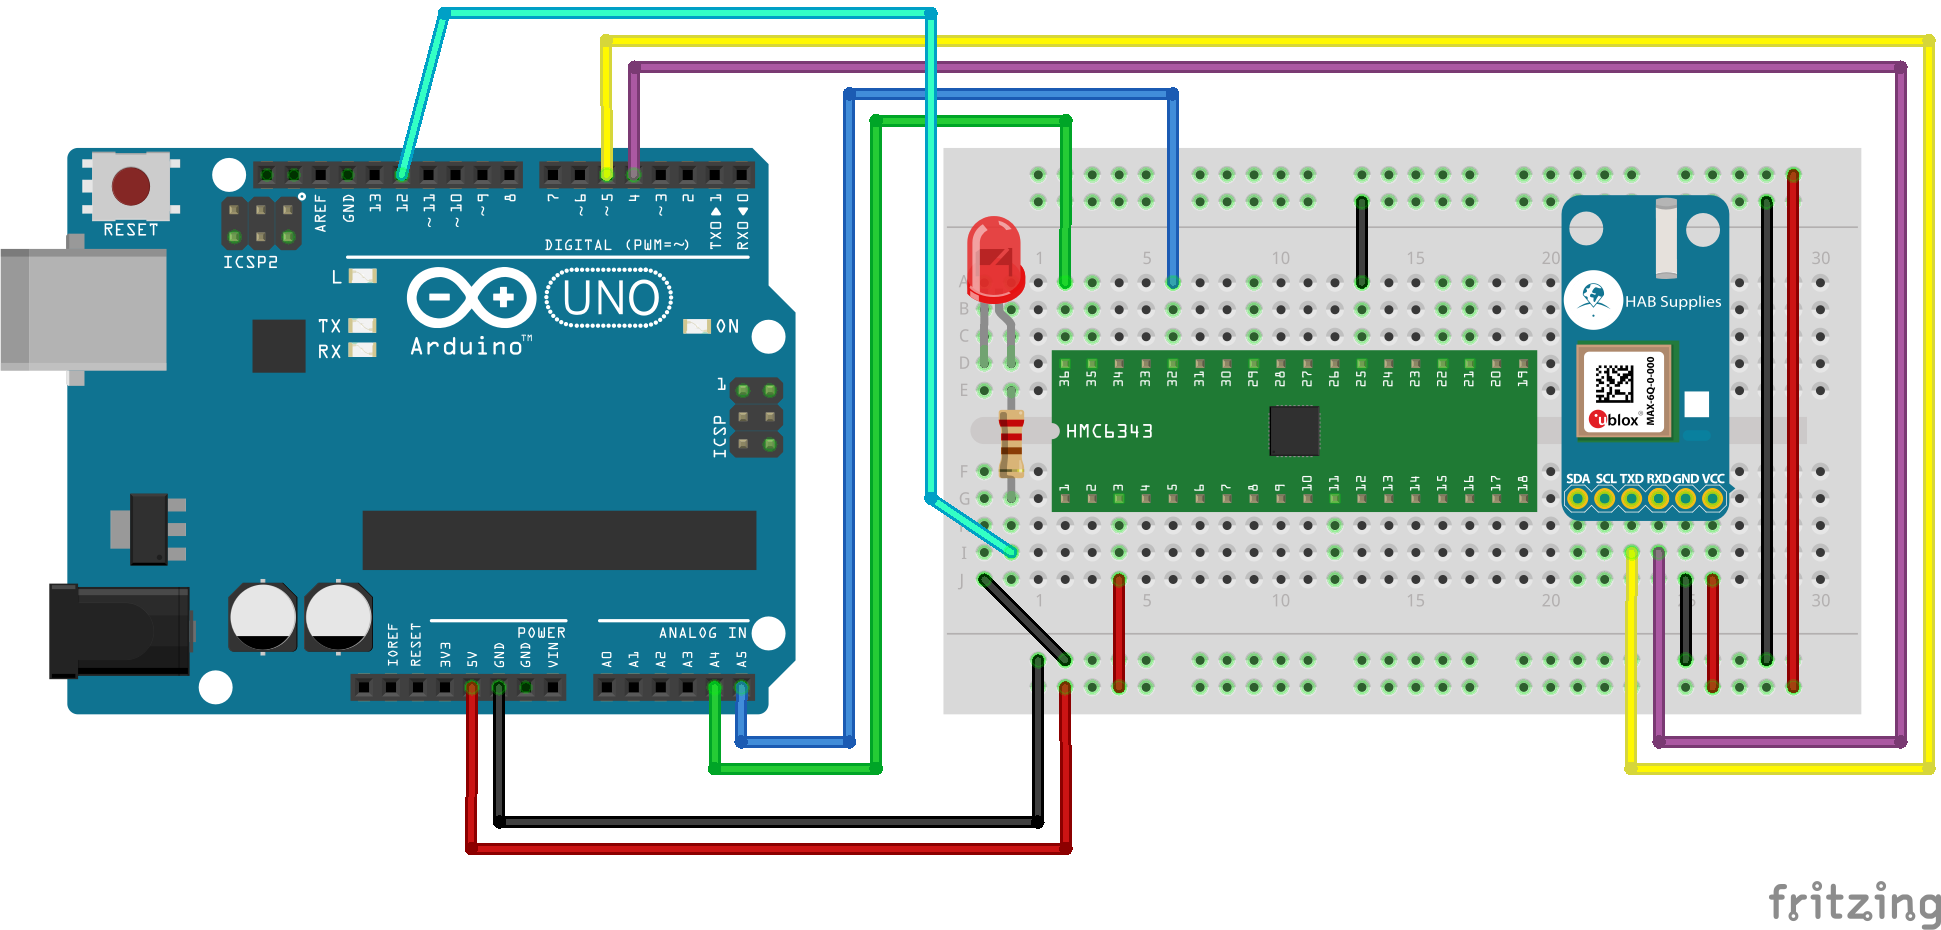
\includegraphics[width=\linewidth]{arduino_wiring_hmc_ublox.png}
  \caption{Example wiring for Arduino with HMC6343 + u-blox MAX-6.}
  \label{arduino_wiring_hmc_ublox.png}
\end{figure}

\begin{figure}[h]
\begin{center}
\begin{minipage}[t]{.47\linewidth}
\begin{center}
\begin{tabular}{| c | c |}
\hline	
\textbf{HMC6343 pin} & \textbf{Arduino Uno R3 pin} \\
\hline
VCC & 5V\HMCvccFootnote{} \\
\hline
GND & GND \\
\hline
SDA & A4\itwocFootnote{} \\
\hline
SCL & A5 \\
\hline
\end{tabular}
\end{center}
\end{minipage}
%
\begin{minipage}[t]{.47\linewidth}
\begin{center}
\begin{tabular}{| c | c |}
\hline	
\textbf{MAX-6 pin} & \textbf{Arduino Uno R3 pin} \\
\hline
VCC & 5V\MAXvccFootnote{} \\
\hline
GND & GND \\
\hline
RXD & D4 \MAXserialFootnote{}\\
\hline
TXD & D5 \\
\hline
\end{tabular}
\end{center}
\end{minipage}
\caption{Pin designation for figure \ref{arduino_wiring_hmc_ublox.png}.}
\label{HMC6343_MAX6_wiringtable}
\end{center}
\end{figure}

Figure \ref{arduino_hmc6343_u-blox_MAX-6.jpg} shows an the assembled unit, comprising an Arduino Uno R3, prototyping shield, HMC6343 \& MAX-6, while figure \ref{pangolin_tablet_back.jpg} shows the packaged unit attached to the back of the WindPad.

\TwoFig{arduino_hmc6343_u-blox_MAX-6.jpg} {Assembled Arduino/sensors.} {arduino_hmc6343_u-blox_MAX-6.jpg}
       {pangolin_tablet_back.jpg} {Arduino/sensors attached to tabet.} {pangolin_tablet_back.jpg}
       
%=========================================================================================================

The MAX-6 is configured as follows;

\begin{enumerate}
	\item Dynamic Platform Model set to Pedestrian.
	\item SBAS via EGNOS is enabled,
	\item GPGLL/GPGSA/GPGSV/GPVTG messages are disabled,
	\item GPRMC/GPGGA messages are enabled.
\end{enumerate}

The Dynamic Platform Models adjust how the navigation engine processes the readings that the receiver produces \& by choosing the correct model for the receiver's application accuracy of position output is increased. As VTW is an application in which the user walks about an outdoor cultural heritage site, the pedestrian model is most suitable. Satellite Based Augmentation System (SBAS) is enabled for the European Geostationary Navigation Overlay Service (EGNOS), which is available at the cultural heritage sites in Scotland that VTW will be used at, to improve the accuracy of the position output.

The output of the receiver is in the form of messages in the NMEA 0183 protocol from the National Marine Electronics Association. By default, the MAX-6 sends many more message types than are required for VTW \& as the Arduino's processing power is limited the superfluous messages are disabled. The GPRMC message format contains the recommended minimum amount of information for transit applications, including time, latitude \& longitude.

These configurations are effected by sending the MAX-6 commands encoded in the UBX protocol as arrays of hex values. For example, setting the Dynamic Platform Model to Pedestrian is performed with the code in figure \ref{arduinoMAX6hex}, where \path{sendUBX} is a function that writes out using SoftwareSerial;

\begin{figure}[h]
\begin{lstlisting}[language=C, numbers=left, numberstyle=\small, stepnumber=1, frame=single, breaklines=true, backgroundcolor=\color{codebackground}, showstringspaces=false]
uint8_t CFG_NAV5[] = {0xB5, 0x62, 0x06, 0x24, 0x24, 0x00, 0xFF, 0xFF,
                      0x03, 0x03, 0x00, 0x00, 0x00, 0x00, 0x10, 0x27,
                      0x00, 0x00, 0x05, 0x00, 0xFA, 0x00, 0xFA, 0x00,
                      0x64, 0x00, 0x2C, 0x01, 0x32, 0x3C, 0x00, 0x00,
                      0x00, 0x00, 0x00, 0x00, 0x00, 0x00, 0x00, 0x00,
                      0x00, 0x00, 0x00, 0x00};
calculateUBXChecksum(CFG_NAV5, (sizeof(CFG_NAV5)/sizeof(uint8_t)));

while (!success)
{
  sendUBX(CFG_NAV5, (sizeof(CFG_NAV5)/sizeof(uint8_t)));
  success = getUBX_ACK(CFG_NAV5);
}
success = 0;
\end{lstlisting}
\caption{Setting MAX-6 Dynamic Platform Model to Pedestrian in an Arduino sketch.}
\label{arduinoMAX6hex}
\end{figure}

These hex arrays can be generated by hand from the UBX protocol specification\maxProtocolFootnote{}, or the MAX-6 can be configured by connecting it directly to a host computer (such as by using an Arduino as an UART by connecting the MAX-6 to digital pins 0 \& 1), configuring the MAX-6 using the u-blox u-center software \& then copying the resultant config as hex messages from the relevant console window.

NMEA messages from the MAX-6 are processed on the Arduino using the TinyGPS library\tinygpsFootnote{}, extracting the latitude \& longitude values before combining them with magnetic compass bearing (yaw) \& pitch values from the HMC6343 \& sending these to the host computer via the Arduino's USB connective.

%=========================================================================================================

\subsection{OpenSim Region Module}

\label{regionModule}

\newcommand{\RegionModuleFootnote}{\footnote{\url{http://opensimulator.org/wiki/IRegionModule}}}

\newcommand{\RegionModuleCodeFootnote}{\footnote{\url{https://bitbucket.org/cj_davies/sharedregionmodulegpsavatar}}}

%=====================

One of the extensions that the OpenSim server provides over the Second Life server that it emulates, is extensibility via Region Modules.

\begin{quotation}
	\textit{``Region modules are .net/mono DLLs. During initialization of the simulator, the OpenSimulator bin directory (bin/) and the scriptengines (bin/ScriptEngines) directory are scanned for DLLs, in an attempt to load region modules stored there. Region modules execute within the heart of the simulator and have access to all its facilities. Typically, region modules register for a number of events, e.g. chat messages, user logins, texture transfers, and take what ever steps are appropriate for the purposes of the module.''}\RegionModuleFootnote{}
\end{quotation}

Region modules allow for more complex \& powerful extensions, written in C\#, to be developed external to the OpenSim platform than would otherwise be possible via Second Life's internal Linden Scripting Language (LSL). Similar to how the Second Life client's joystick interface represented an opportunity to implement the orientation control of VTW without relying upon a bespoke, modified client, an OpenSim Region Module represents the possibility to implement the position control required by VTW without relying upon a similarly bespoke client.

An excerpt from the implementation of the position control required by VTW is included as \ref{RegionModuleCode1} (full Region Module code available online\RegionModuleCodeFootnote{}). This shows the use of haversine, implemented using the \texttt{atan2()} function, calculating the displacement in real world latitude between the anchor point \& the new GPS reading (lines 5-8), applying the scale of the reconstruction to this displacement (lines 10-14) \& then applying this scaled displacement to the virtual world Y coordinate of the anchor (lines 16-24). This process is then repeated for the longitude/X coordinate \& the avatar can then be moved to the position within the OpenSim reconstruction that is equivalent to the user's new real world position.

\begin{figure}[h]
\begin{lstlisting}[language=Java, numbers=left, numberstyle=\small, stepnumber=1, frame=single, breaklines=true, backgroundcolor=\color{codebackground}, showstringspaces=false]
private Vector3 LatitudeLongitudeToRegionCoordinate(double newLat, double newLong, double anchorLat, double anchorLong, Vector3 anchorVector, double scale) {

    double d, a, c, X, Y;

    //calculate the difference in y (latitude) between the anchor & the new reading
    d = Math.Abs(ToRadians(newLat - anchorLat));
    a = Math.Sin(d / 2) * Math.Sin(d / 2);
    c = 2 * Math.Atan2(Math.Sqrt(a), Math.Sqrt(1 - a));

    //mean radius of the Earth is 6371km (6371000m)
    d = 6371000 * c;

    //apply scale
    d *= scale;

    //sum appropriately from the anchor
    if (newLat > anchorLat) {
        mlog.DebugFormat("[GPSAvatarModule]: LatitudeLongitudeToRegionCoordinate() - (Y) newLat > anchorLat.");
        Y = (anchorVector.Y + d);
    }
    else {
        mlog.DebugFormat("[GPSAvatarModule]: LatitudeLongitudeToRegionCoordinate() - (Y) newLat < anchorLat.");
        Y = (anchorVector.Y - d);
    }
\end{lstlisting}
\caption{Excerpt of OpenSim Region Module for avatar movement via GPS.}
\label{RegionModuleCode1}
\end{figure}

%=========================================================================================================

%\clearpage

%=========================================================================================================

\section{Modifying Second Life for Orientation \& Position Control}

Due to the Second Life client's existing control interfaces not allowing enough control over camera orientation for VTW's requirements (section \ref{exploitJoystick}), it was necessary to modify the client's codebase to produce a bespoke client allowing complete control over orientation by magnetometer \& accelerometer input. Although sufficient position control could be achieved via an OpenSim region module (section \ref{regionModule}) it was prudent to also encapsulate position control through the modified client; not only does this allow for finer grain control, it also removes the dependency upon the virtual reconstruction being hosted upon an OpenSim server (Second Life's own servers do not support extension via Region Modules). Thus, the Second Life client was modified with the addition of the ability to;

\begin{itemize}
	\item connect to a serial device for I/O,
	\item control movement of the avatar according to input from this serial device,
	\item control the camera according to input from this serial device.
\end{itemize}

%=========================================================================================================

\subsection{Overview of Second Life Client Modifications}

\newcommand{\asioFootnote}{\footnote{\url{http://www.boost.org/doc/libs/1_57_0/doc/html/boost_asio.html}}}

\newcommand{\boostFootnote}{\footnote{\url{http://www.boost.org/}}}

\newcommand{\fedetftFootnote}{\footnote{\url{http://www.webalice.it/fede.tft/serial_port/serial_port.html}}}

\newcommand{\regionmodulelimitationFootnote}{\footnote{This is not due to any limitation on the part of OpenSim, but simply due to the Second Life client modifications being pursued further than the OpenSim module.}}

\newcommand{\megaregionFootnote}{\footnote{\url{http://opensimulator.org/wiki/Setting_Up_Mega-Regions}}}

%=====================

%Replaced the Linden Boost binary with that built by LightDrake

The Second Life client is written predominantly in C++ so the Asio library\asioFootnote{} from the popular Boost project\boostFootnote{} is used to imbue it with serial connectivity, allowing it to receive messages from the Arduino in an asynchronous non-blocking fashion. The fundamental buffered asynchronous serial handling is implemented using Terraneo Federico's \path{AsyncSerial} class\fedetftFootnote{} which is included in the client codebase as \path{/indra/newview/AsyncSerial}. The majority of the functionality added to the client is then contained within \path{/indra/newview/LLViewerSerialMovement}. The core executable of the viewer, \path{/indra/newview/LLAppViewer} obtains an instance of \path{LLViewerSerialMovement} \& then calls \path{LLViewerSerialMovement::update()} upon each iteration of the client's main update loop, \path{LLAppViewer::mainLoop()}. These modifications are visualised by figure \ref{second_life_structure.png}.

\begin{figure}[h]
\centering
  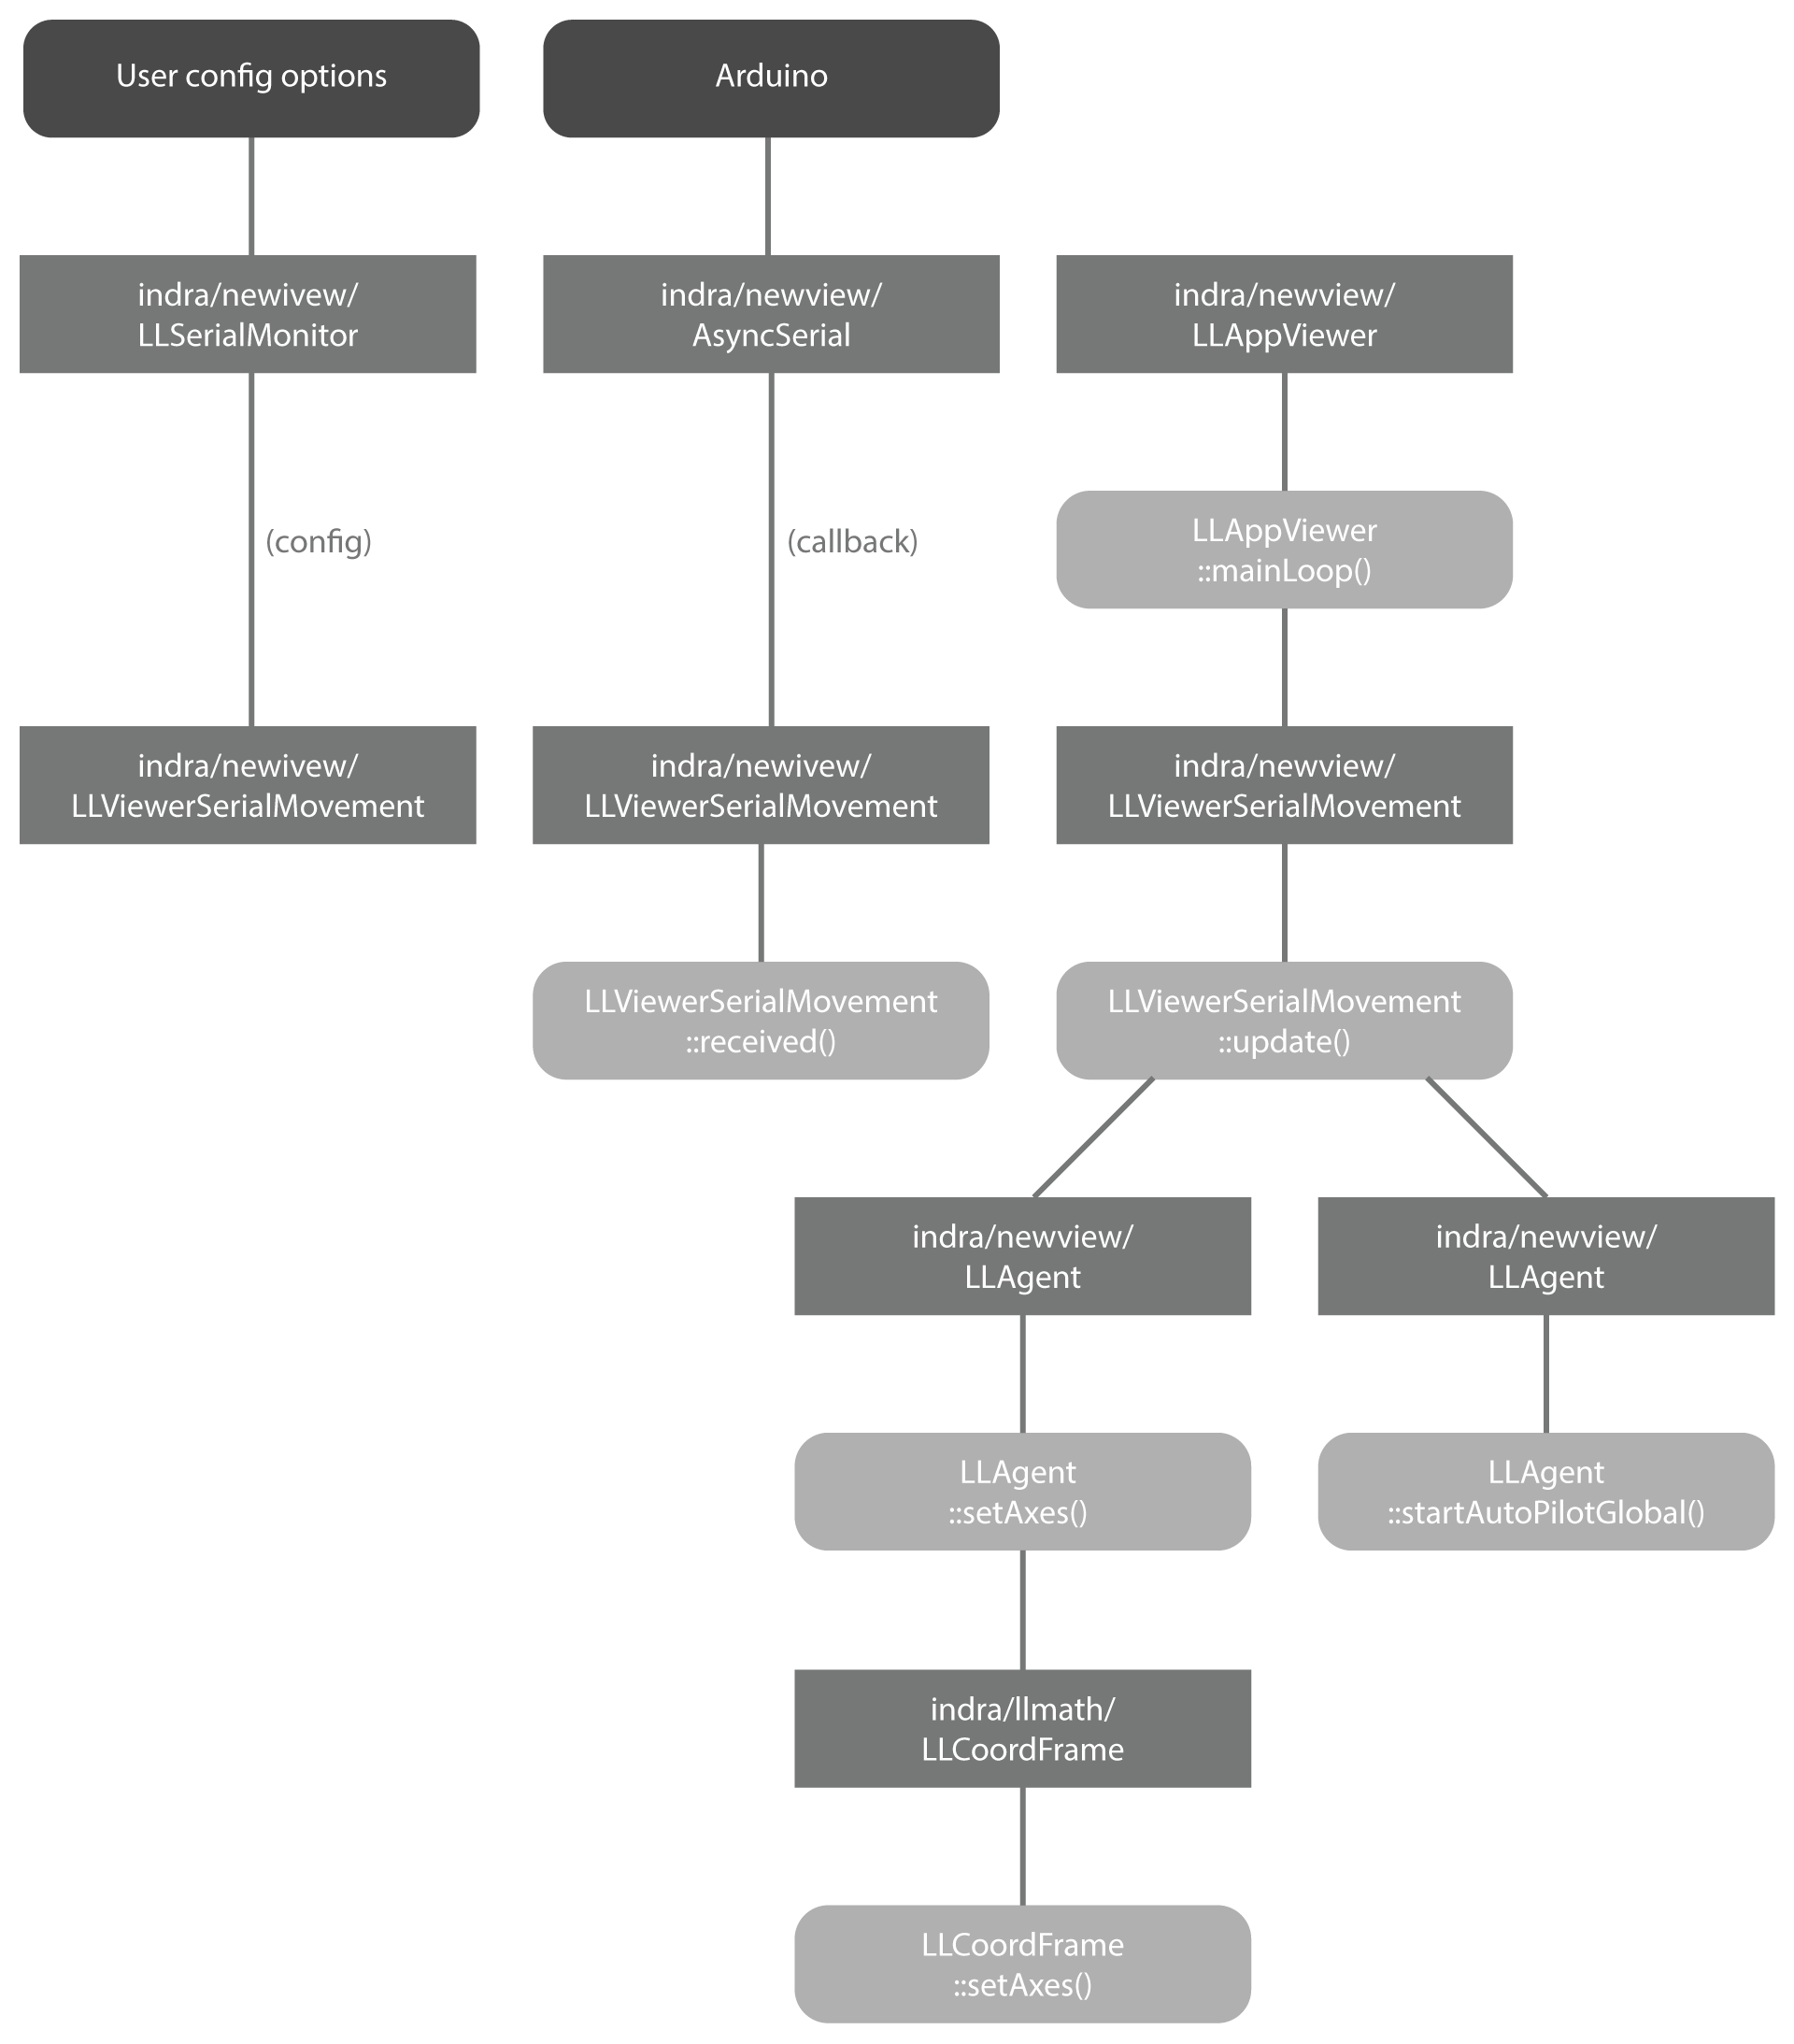
\includegraphics[width=.8\linewidth]{second_life_structure.png}
  \caption{Overview of modifications to Second Life client.}
  \label{second_life_structure.png}
\end{figure}

%=========================================================================================================

\subsection{\texttt{LLViewerSerialMovement} reference}
Brief documentation of the functions in \path{/indra/newview/LLViewerSerialMovement} follows.
\begin{center}
\begin{longtable}{| p{4.2cm} | p{10cm} |}

\hline	
	
%=========================================================================================================
		
\texttt{::connect} & Safely connects to a serial device (if not already connected). \\
		
\hline

%=========================================================================================================

\texttt{::disconnect} & Safely disconnects from a serial device (if already connected). \\
		
\hline

%=========================================================================================================

\texttt{::received} & A callback method registered to the \path{CallbackAsyncSerial} class in \path{/indra/newview/AsyncSerial}. This function parses the data (\path{const} \path{char} \path{*data}) from the serial device, extracting complete messages to the variable \path{mostRecentMessage}. Because of the nature of the serial I/O, \path{*data} is not guaranteed to contain a discrete message from the Arduino containing both orientation \& position data, thus this function must parse the array \& assemble discrete messages from possibly multiple subsequent callbacks. \\
		
\hline

%=========================================================================================================

\texttt{::update} & Called upon each iteration of \path{LLAppViwer::mainLoop()} \& further calls \path{::updateFromMostRecentMessage()}, \path{::updateOrientation()} \& \path{::updatePosition()}. \\
		
\hline

%=========================================================================================================

\texttt{::updateFromMostRecent- Message} & Processes a complete message from the Arduino which has been assembled by \path{::received()} \& extracts the constituent orientation \& position values. \\
		
\hline

%=========================================================================================================

\texttt{::updateOrientation} & Applies the orientation values extracted from an Arduino message to the avatar's camera. This is achieved by a call to \path{LLAgent::setAxes()} which calls \path{LLCoordFrame::setAxes()} in \path{/indra/llmath/LLCoordFrame}. The orientation values are passed as a quaternion, converting the bearing, pitch \& roll values extracted from the Arduino message as degrees using \path{::quaternionFromDegrees()}.\\
		
\hline

%=========================================================================================================

\texttt{::updatePosition} & Applies the position data extracted from an Arduino message to the avatar, using \path{LLAgent::startAutoPilotGlobal()} to perform smooth movement between the avatar's current position (obtained with \path{LLAgent::getPositionGlobal()}) \& the new position from the Arduino (converted from latitude \& longitude to Second Life region coordinates in \path{::latitudeLongitudeToRegionCoordinates()}). \\
		
\hline

%=========================================================================================================

\texttt{::quaternionFromDegrees} & A helper method to convert bearing, pitch \& roll expressed in degrees, into a single quaternion. Quaternions are frequently used to represent rotations in 3D applications, as they do not suffer from gimbal lock - Second Life is no exception to this \& internally uses quaternions for all rotation data, providing \path{/indra/llmath/LLQuaternion} for this purpose. \\
		
\hline

%=========================================================================================================

\texttt{::latitudeLongitudeTo- RegionCoordinate} & Converts a real world position, expressed as a longitude \& latitude pair, to the equivalent Second Life coordinates, applying the haversine formula using knowledge of the real world \& corresponding Second Life position of the anchor point \& the scale of the Second Life reconstruction compared to the real world. \\
		
\hline

%=========================================================================================================

\texttt{::degreesToRadians} & A helper method to convert values expressed in degrees to the equivalent value expressed in radians (implementations of the haversine formula usually make use of radians). \\
		
\hline

%=========================================================================================================

\end{longtable}
\end{center}

%=========================================================================================================

Controlling the avatar's position according to latitude \& longitude readings from the GPS receiver is once again implemented using the haversine formula. This implementation, included as figure \ref{secondlifehaversine} can be compared to the OpenSim region module version included previously as figure \ref{RegionModuleCode1}. One important difference between the Second Life client implementation \& the OpenSim region module implementation is that the former uses global coordinates, rather than local coordinates\regionmodulelimitationFootnote{}. This means that the Second Life client implementation allows positional control of an avatar across region boundaries, crucial for use with a cultural heritage reconstruction that spans multiple regions in an OpenSim `megaregion'\megaregionFootnote{} such as that used for testing of VTW.

These modifications to the Second Life client are configured/controlled via a window added to the client \& accessed via a menu entry (see figure \ref{pangolin_second_life_dialogue.png}). The implementation of this resides in \path{/indra/newview/LLViewerSerialMonitor}. This allows for specification of the path to the serial device, along with its baudrate, as well as the specification of the anchor point - the latitude \& longitude of the point in the real world \& the equivalent X/Y coordinates in the Second Life reconstruction. The window then provides diagnostic output showing the messages coming in from the serial device, along with controls to individually enable/disable orientation \& position control \& alter the high-pass \& smoothing applied to both controls.

\begin{figure}[h]
\centering
  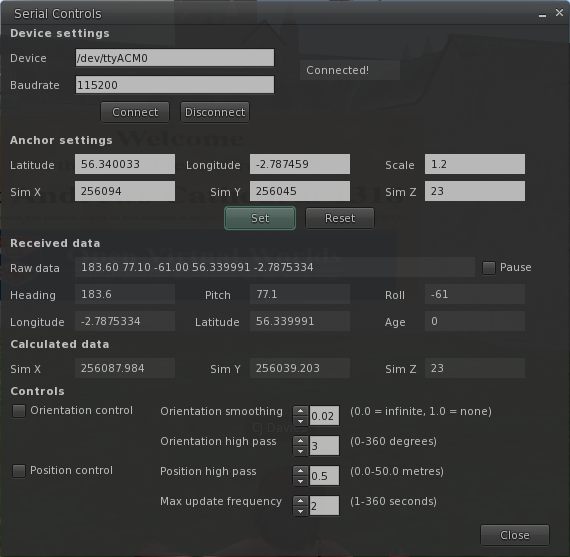
\includegraphics[width=0.6\linewidth]{pangolin_second_life_dialogue.png}
  \caption{Config pane in modified Second Life client for HMC6343 + MAX-6.}
  \label{pangolin_second_life_dialogue.png}
\end{figure}

\begin{figure}[h]
\begin{lstlisting}[language=C++, numbers=left, numberstyle=\small, stepnumber=1, frame=single, breaklines=true, backgroundcolor=\color{codebackground}, showstringspaces=false]
boost::tuple<float, float, float> LLViewerSerialMovement::latitudeLongitudeToRegionCoordinate(double newLat, double newLong, float anchorLat, float anchorLong, float scale, boost::tuple<float, float, float> anchorCoordinates) {

    double d, a, c, X, Y;

    // calculate difference in y (latitude) between anchor & new reading
    d = fabs(degreesToRadians(newLat - anchorLat));
    a = sin(d / 2) * sin(d / 2);
    c = 2 * atan2(sqrt(a), sqrt(1 - a));

    // mean radius of the Earth is 6371km (6371000m)
    d = 6371000 * c;

    // apply scale
    d *= scale;

    // sum appropriately from the anchor
    if (newLat > anchorLat) {
        Y = (anchorCoordinates.get<1>() + d);
    }
    else {
        Y = (anchorCoordinates.get<1>() - d);
    }

    // calculate difference in x (longitude) between anchor & new reading
    d = fabs(degreesToRadians((newLong - anchorLong)));
    a = sin(d / 2) * sin(d / 2) * cos(degreesToRadians(newLat)) * cos(degreesToRadians(anchorLat));
    c = 2 * atan2(sqrt(a), sqrt(1 - a));
    
    d = 6371000 * c;

    // apply scale
    d *= scale;

    // sum appropriately from anchor
    if (newLong > anchorLong) {
        X = (anchorCoordinates.get<0>() + d);
    }
    else {
        X = (anchorCoordinates.get<0>() - d);
    }

    return boost::make_tuple(X, Y, anchorCoordinates.get<2>());
}
\end{lstlisting}
\caption{Converting longitude \& latitude to Second Life coordinates using haversine.}
\label{secondlifehaversine}
\end{figure}

%=========================================================================================================

\clearpage

%=========================================================================================================

\section{VTW in Use}

\newcommand{\thinkpadFootnote}{\footnote{\url{http://support.lenovo.com/us/en/documents/pd012148}}}

\newcommand{\wrtFootnote}{\footnote{\url{http://support.linksys.com/en-eu/support/routers/WRT54G}}}

%=====================

The backdrop for real world experimentation with the VTW platform was the impressive ruins of St Andrews cathedral.

\begin{figure}[h]
\centering
  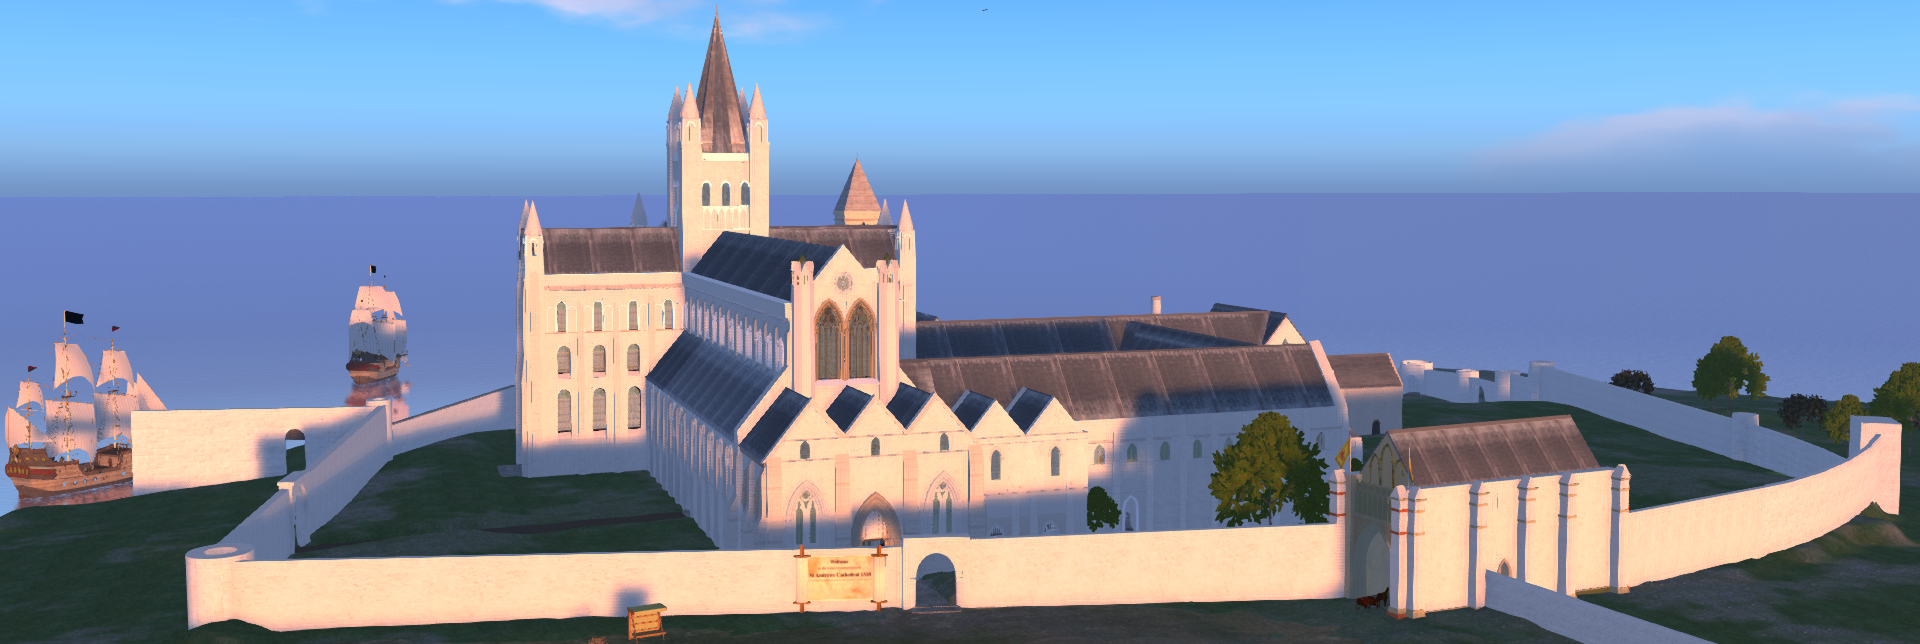
\includegraphics[width=\linewidth]{cathedral_reconstruction_side.png}
  \caption{St Andrews Cathedral recreation set on the sunny St Andrews day afternoon 1318, showing the West Gate in the foreground \& ships in the background.}
  \label{cathedral_reconstruction_side.png}
\end{figure}

%=====================

%~\cite{Kennedy2013} Canons \& Cathedrals

St Andrews Cathedral occupies a site used for worship since the 8th Century AD. Work on the Cathedral began around 1160 and was completed nearly 150 years later (the west fa\c{c}ade and parts of the nave collapsed in a storm around 1270). It was finally consecrated in 1318 four years after the battle of Bannockburn and in the presence of King Robert I of Scotland. St Andrews Cathedral was in its prime, the centre of Scotland’s religious life, its largest and most magnificent church. In 1378 the Cathedral suffered a significant fire prompting
a reworking of many of its features including the West and East End windows. Its presence was the catalyst for the foundation of a university at St Andrews in the early fifteenth century~\cite{Fawcett2011}, which remains an important seat of learning to this day. In 1561 following the Scottish reformation the Cathedral was abandoned by the Bishops and replaced by the parish church as the chief place of worship. The former headquarters of the Scottish Church was left to fall into ruin, with much of its stone being used in the construction of town dwellings.

During its time the Cathedral was central to Scottish personalities and history. St Andrews was the highest ranking Scottish see. The establishment of Augustinian Cannons followed by the initiation of
building work by Bishop Ernald reflected integration with the European church, economic dynamism and decline of the Celtic Church. The diocese funded Robert Bruce during the Wars of Independence. Its Bishop William de Lamberton contributed to the formulation of the Declaration of Arbroath, a central document in the formation of
Scottish Nationhood. Isabella, sister of Donnchadh IV, last Pictish Earl of Fife, crowned Bruce King. John Knox personally lead his congregation against the Cathedral’s finery and following the murder of Cardinal Beaton the first Scottish protestant congregation was established in the Bishop’s palace.

Important fragments of the remain. The east gable of the presbytery, where the relics of St Andrew were purported to be kept, along with the south wall of the nave, and the majestic West Entrance all point to the Cathedral’s former majesty. The cloister retains its ruined chapter house and stone-vaulted under crofts. Consequently, much evidence of the Cathedral’s form exists. A view from the nave looking towards the choir in figure \ref{cathedral_real_outside.jpg}.

%=====================

The OVW Group's reconstruction of St Andrews cathedral, as shown in figures \ref{cathedral_reconstruction_side.png} \& \ref{cathedral_reconstruction_above.jpg}, represents the site as it stood in 1318, the year of its consecration. This virtual reconstruction, presenting a historically accurate model of the cathedral as it stood at the peak of its former glory, is very large at over 400m by 600m \& spanning multiple storeys, featuring the cloisters as well as the Cannons' living quarters.

\TwoFig{cathedral_real_outside.jpg} {St Andrews cathedral today.} {cathedral_real_outside.jpg}
       {cathedral_reconstruction_above.jpg} {St Andrews cathedral reconstruction.} {cathedral_reconstruction_above.jpg}

%=========================================================================================================

\subsection{Experimental Implementation}
For the purposes of testing VTW at the cathedral, a temporary server \& network setup was effected using a Lenovo ThinkPad X61s\thinkpadFootnote{} laptop computer to host the OpenSim server with a Linksys WRT54G\wrtFootnote{} wireless router powered from a 12V sealed lead-acid battery to provide wireless communication between the OpenSim server \& the WindPad over a much larger range than the laptop's internal wireless interface could provide. This setup is shown in use at the cathedral by figure \ref{server} \& the architecture of this experimental implementation is shown by figure \ref{vtw_implementation.png}.

\TwoFig{pangolin_laptop_router_battery.jpg} {OpenSim Server \& wireless AP.} {pangolin_laptop_router_battery.jpg}
       {pangolin_in_use.jpg} {VTW at the cathedral.} {pangolin_in_use.jpg}

\begin{figure}[h]
\centering
  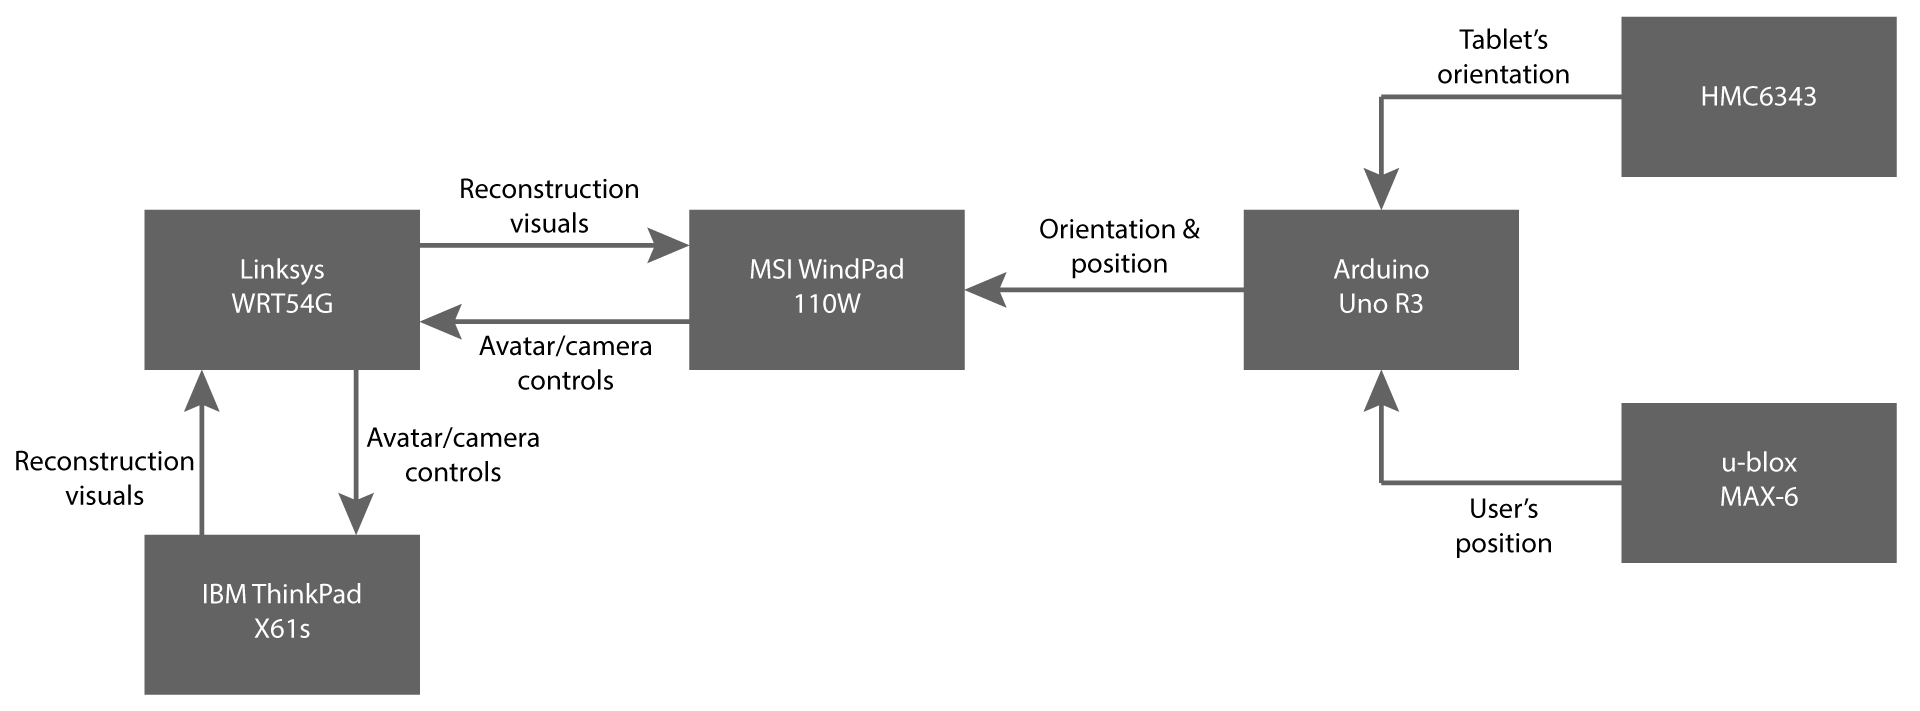
\includegraphics[width=\linewidth]{vtw_implementation.png}
  \caption{Implementation of VTW.}
  \label{vtw_implementation.png}
\end{figure}

%=========================================================================================================

\textbf{***Go through Arduino sketch \& talk about things like magnetic declination, etc.}

%Magnetic declination information was entered into the HMC6343 for the position of the cathedral and the date of our experiments. The HMC6343's hard-iron offset calculation feature was used each time the hardware configuration was altered. The sampling frequency of the HMC6343 was set to its highest value of 10Hz. Orientation was set to `upright front' to match the physical orientation of the IC in the experiments.


%The MAX-6 was operated in `pedestrian' dynamic platform model, use of SBAS correction data was enabled and frequency of readings was set to the maximum of 5Hz.

%=========================================================================================================

\subsection{Real World Performance of VTW}

\newcommand{\ubloxcepFootnote}{\footnote{\url{https://u-blox.com/images/downloads/Product_Docs/MAX-6_ProductSummary_(GPS.G6-HW-10089).pdf}}}

%=====================

The product summary for the MAX-6 claims accuracy of 2.5m Circular Error Probable (CEP) without SBAS corrections and 2m CEP with SBAS corrections \textit{``demonstrated with a good active antenna''}\ubloxcepFootnote{}. This means that, in an ideal situation with SBAS correction data available, there would be 50\% certainty that each position reported by the GPS receiver would be within 2m of its actual position. The SL-1202 antenna used is passive, however as the distance between antenna and the MAX-6 IC itself in the hardware application is only a few millimeters there would have been negligible benefit from using an active antenna. However whether the SL-1202 constitutes `good' for achieving the headlining performance characteristics of the MAX-6 is debatable as the definition of `good' was not provided in the product summary.


To determine the real world accuracy attainable with the MAX-6 outfitted with the SL-1202 in situations akin to those of the cultural heritage case study, a walking route around the St Andrews cathedral ruins, akin to the route that an individual visitor or school group might take, was planned and then walked with the MAX-6 connected to a laptop computer via an Arduino operating as a Universal Asynchronous Receiver/Transmitter (UART) feeding the raw National Marine Electronics Association (NMEA) messages into the `u-center'GPS evaluation software version 7.0 which logged the messages for later evaluation. Simultaneously for comparative purposes a mid-range consumer Android smartphone was used to record the same track; a HTC One S~\cite{HTCCorporation2013} containing a gpsOne Gen 8A solution within its Qualcomm Snapdragon S4 processor~\cite{QualcommIncorporated2013} and using Google's `My Tracks' app version 2.0.3 to record the data. The three sets of positional data (planned route, MAX-6 recorded route and smartphone recorded route) were entered into a PostgreSQL database~\cite{Daviesc,Daviesb} and the PostGIS database extender's ST\_HausdorffDistance algorithm~\cite{PostGIS} was used to calculate the Hausdorff distances between the recorded routes and the planned route and between the recorded routes themselves. In this scenario, the Hausdorff distance represents the furthest distance needed to travel from any point on the route recorded by the GPS receiver to reach the nearest point on the planned route. Because of the substantially greater inaccuracies identified in the latter part of the recorded tracks, separate Hausdorff distances were calculated both for the complete tracks and also for truncated first and second sub-tracks.

This ability to control navigation within the 3D virtual environment without explicit conscious input of keyboard/mouse/touch commands is integral to reducing the cognitive load required to maintain a presence within a virtual environment which is a key requirement for overcoming the vacancy problem and achieving successful mobile cross reality.

During the experiments the MAX-6 was unable to maintain reception of the additional correction data required for SBAS operation; when left stationary for several minutes reception was possible however subsequent movement of only a few meters at walking pace broke the connection. This reduced the theoretical maximum performance of the unit to 2.5m CEP, with observed performance being lower. Figure \ref{map_one} depicts an aerial view of the St Andrews cathedral ruins; the blue line represents the planned route, red the route recorded by the MAX-6 receiver and green the route recorded by the smartphone for comparative purposes, both while walking the planned route.

%\begin{figure}[h]
%\centering
%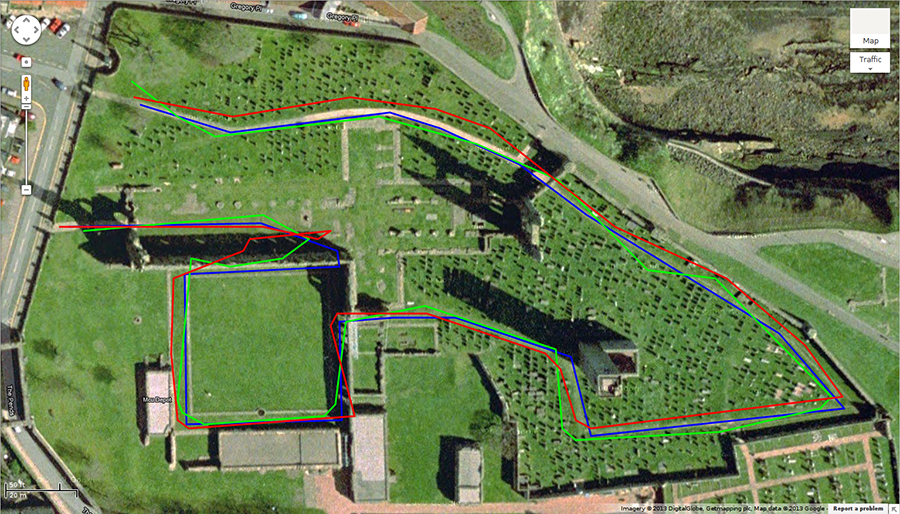
\includegraphics[width=0.48\textwidth]{images/figure_4}
%\caption{Aerial view oriented North upward of the St Andrews cathedral ruins; the blue line represents the planned route, red the route recorded by the MAX-6 and green the route recorded by the smartphone whilst walking the planned route.}
%\label{map_one}
%\end{figure}

The Hausdorff distance between the planned route and that recorded by the MAX-6 was $1.02e^{-04\circ}$. The `length' of a degree of latitude and a degree of longitude depends upon location upon the Earth; around the location of the St Andrews cathedral 1$^\circ$ of latitude is equivalent to 111347.95m and 1$^\circ$ of longitude to 61843.88m. Thus the Hausdorff distance of $1.02e^{-04\circ}$ can be visualized as $\pm11.3$m of North/South inaccuracy or $\pm6.3$m of East/West inaccuracy (or a combination of both N/S and E/W inaccuracy not exceeding a total displacement of $1.02e^{-04\circ}$ from the planned route).

The MAX-6 did achieve better performance than the smartphone, which recorded a Hausdorff distance of $1.33e^{-04\circ}$ ($\pm14.8$m N/S, $\pm8.2$m E/W). The Hausdorff distance between the routes logged by the MAX-6 and the smartphone was $1.14e^{-04\circ}$ ($\pm12.7$m N/S, $\pm7.0$m E/W), which represents a low correlation between the inaccuracies recorded by the two receivers even though they are of similar magnitudes from the planned route.

The maximum inaccuracies were recorded when walking along the South wall of the cathedral's nave. This wall is one of the most complete sections of the building with stonework reaching some 30ft above ground level and providing an effective obstruction to line-of-sight to half of the sky (and substantially impairing reception of signals from GPS satellites) when in close proximity to it. When considering just the sub-route shown in figure \ref{map_two}, which terminates before this wall begins to significantly obstruct view of the sky, the Hausdorff distances are notably smaller; the MAX-6 achieved a Hausdorff distance of $7.23e^{-05\circ}$ ($\pm8.05$m N/S, $\pm4.47$m E/W) throughout this sub-route, with the smartphone still behind with $8.99e^{-05\circ}$ ($\pm10.01$m N/S, $\pm5.56$m E/W). Again the Hausforff distance between the receivers showed low correlation between the inaccuracies, at $6.43e^{-05\circ}$ ($\pm7.12$m N/S, $\pm3.98$m E/W).
 
%\begin{figure}[h]
%\centering
%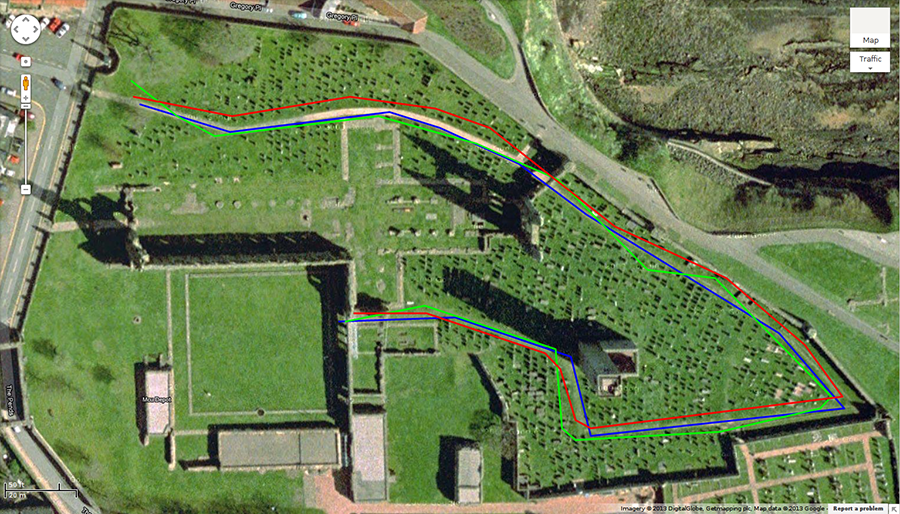
\includegraphics[width=0.48\textwidth]{images/figure_5}
%\caption{Aerial view oriented North upward of the St Andrews cathedral ruins; the blue line represents the first sub-route of the planned route, red the sub-route recorded by the MAX-6 and green the sub-route recorded by the smartphone whilst walking the first planned sub-route.}
%\label{map_two}
%\end{figure}

When analyzing the tracks in the vicinity of the nave (see figure \ref{map_three}) it is shown that although the MAX-6 outperformed the smartphone in terms of Hausdorff distance this relationship can be considered misleading as the smartphone track corresponded more closely in shape to the planned route even if it did stray further at its extreme. The discrepancy in the behavior of the two receivers in this situation is attributed to different implementations of dead-reckoning functionality between the receivers. Dead-reckoning is the process used when a GPS receiver loses reception of location data from satellites and extrapolates its position based upon a combination of the last received position data and the velocity of travel at the time of receiving these data.
 
%\begin{figure}[h]
%\centering
%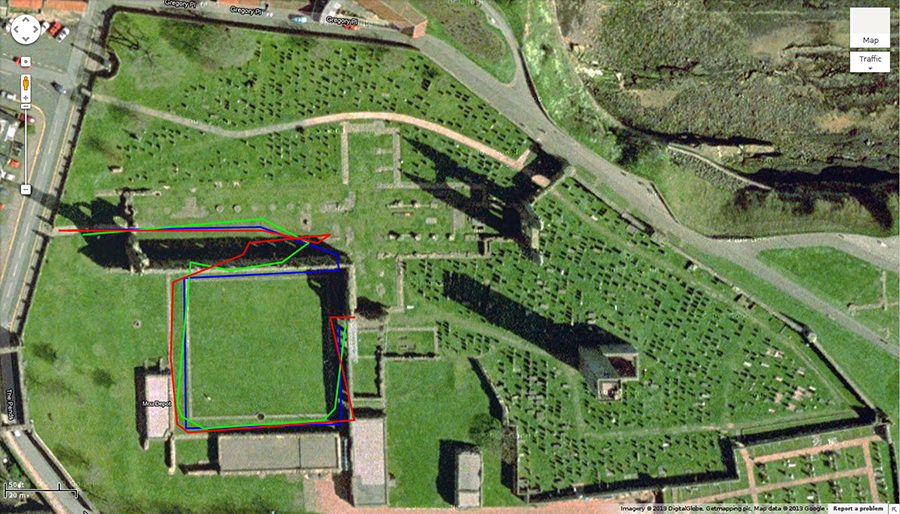
\includegraphics[width=0.48\textwidth]{images/figure_6}
%\caption{Aerial view oriented North upward of the St Andrews cathedral ruins; the blue line represents the second sub-route of the planned route, red the sub-route recorded by the MAX-6 and green the sub-route recorded by the smartphone whilst walking the second planned sub-route.}
%\label{map_three}
%\end{figure}

Pangolin's camera control from orientation data does not have as stringent performance criteria as the movement control from position data. Unlike augmented reality where sparse virtual content is superimposed upon a view of a real environment and the virtual objects must be placed accurately in order for the effect to work well, cross reality presents a complete virtual environment that is viewed `separately' or side-by-side with the real environment and thus discrepancies between orientation of real and virtual environments have a less detrimental effect to the experience. Although the accuracy of the camera control during the experiments was reported as being sufficient, the speed at which the camera orientation moved to match physical orientation was reported as being too slow, resulting in having to wait for the display to `catch up' to changes in orientation. This is attributed to the 10Hz sampling rate of the orientation sensors which, particularly after readings are combined for smoothing purposes to reduce jerky movement, resulted in too infrequent orientation updates. Frame rates within Pangolin whilst navigating the route averaged between 15 and 20 frames per second with the viewer's `quality and speed' slider set to the `low' position.

The style of explorative interaction with virtual content that this system employs is more resilient to input lag and low frame rates than other scenarios of interaction with virtual content such as fast paced competitive video games including First Person Shooters (FPS) [20], but overall user experience would nonetheless be improved by a faster sampling of orientation data and a higher frame rate. Additionally it should be noted that the cathedral reconstruction was created with relatively powerful desktop computers in mind as the primary deployment platform and has not been optimized for use on less powerful mobile platforms such as Pangolin. Performance of Pangolin on a less graphically complex OpenSim region (Salt Pan 2 [17]), that also depicts a reconstruction of a cultural heritage site, was better at 20 to 25 frames per second at the `low' position and between 15 and 20 frames per second at `high' (see figure 7).

%\begin{figure}[h]
%\centering
%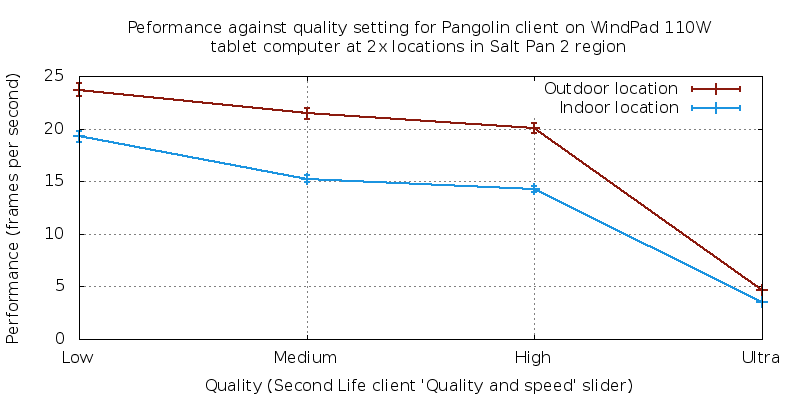
\includegraphics[width=0.48\textwidth]{images/figure_7}
%\caption{Plot of Pangolin's performance (measured in frames per second) against different graphical settings (selected via the `Quality and speed' slider of the viewer) in two positions within the Salt Pan 2 region.}
%\label{framerate_graph}
%\end{figure}

%\section{Interpretations}
The positional accuracy of $1.02e^{-04\circ}$ attained by the MAX-6 is sufficient for the first modality of interaction (that of distinguishing and navigating between multiple points of interest). This value of $1.02e^{-04\circ}$ (analogous to a combination of $\pm11.3$m of North/South inaccuracy or $\pm6.3$m of East/West inaccuracy) represents a constraint on the granularity of the content; it is the minimum distance required between any two points of interest for them to be correctly differentiated between. This same value is not sufficient for the second modality of interaction (that of free roaming exploration with avatars mimicking their users' movements as closely as possible). This modality would require the use of additional position tracking techniques to improve accuracy to around 1m CEP (analogous to $8.98e^{-06\circ}$ latitude or $1.62e^{-05\circ}$ longitude around the location of the St Andrews cathedral).

Use of a GPS receiver that is lower performance than the MAX-6 used by Pangolin, but more common due to being of the calibre integrated into smartphones and tablets such as that used in the experiments, is still sufficient for the first modality but with a larger minimum distance required between any two points of interest. The Hausdorff distance of $1.33e^{-04\circ}$ recorded by the smartphone used in the experiments is analogous to $\pm14.8$m N/S or $\pm8.2$m E/W around the location of the cathedral.

Observed accuracy of the orientation tracking is sufficient for both modalities of interaction; the accuracy of orientation tracking required does not change with different positional accuracy and the accuracy of orientation attained in the experiments is sufficient for an acceptable user experience, however the experience would benefit from better graphical quality and higher responsiveness to changes in user orientation.

%=========================================================================================================

\section{Using the Virtual Time Window}

Two plausible modalities of interaction were identified for this system, with each presenting different requirements with regards to accuracy of position tracking.

The first modality is one in which a number of locations that represent points of particular interest are identified. This is already a common practice at cultural heritage sites, with such locations often bearing signs or placards presenting text and/or images explaining what can be observed from the position. With Pangolin, when a user walks within a certain range of such a point, their avatar can be moved to the corresponding location within the reconstruction (and a sound played to alert the user to the fact that there is something of interest to observe) from which they can then move the tablet around them to examine their surroundings in the reconstruction. This modality is similar to audio tours employed by many museums and cultural heritage sites, but replaces the requirement to follow a static route or type in numbers of locations with the ability to freely navigate the real environment with access to additional information being triggered automatically once within the required range of a point of interest.

The second modality is one of free roaming exploration, in which the movements of the user's avatar within the reconstruction mimic the user's movements within the real world as closely as possible.
The first modality can be scaled to function with different accuracies of position tracking; as long as the distance between any two points of interest is at least as much as the worst case performance of the position tracking then distinguishing correctly between different points will always succeed. The second modality requires extremely accurate position tracking, arguably surpassing the capabilities of mainstream GPS technology even in ideal situations.

%=========================================================================================================